\section{Helium-3/Deuterium Yield Ratio}

The Helium-3/Deuterium yield ratio was calculated using the analysis method outlined in Section \ref{sec:analysis_outline}. The data is shown in Figure \ref{fig:yr1} and listed in Table \ref{tbl:fy1}. The uncertainties plotted consist of statistical and all systematic uncertainties.

\begin{figure}[p]
	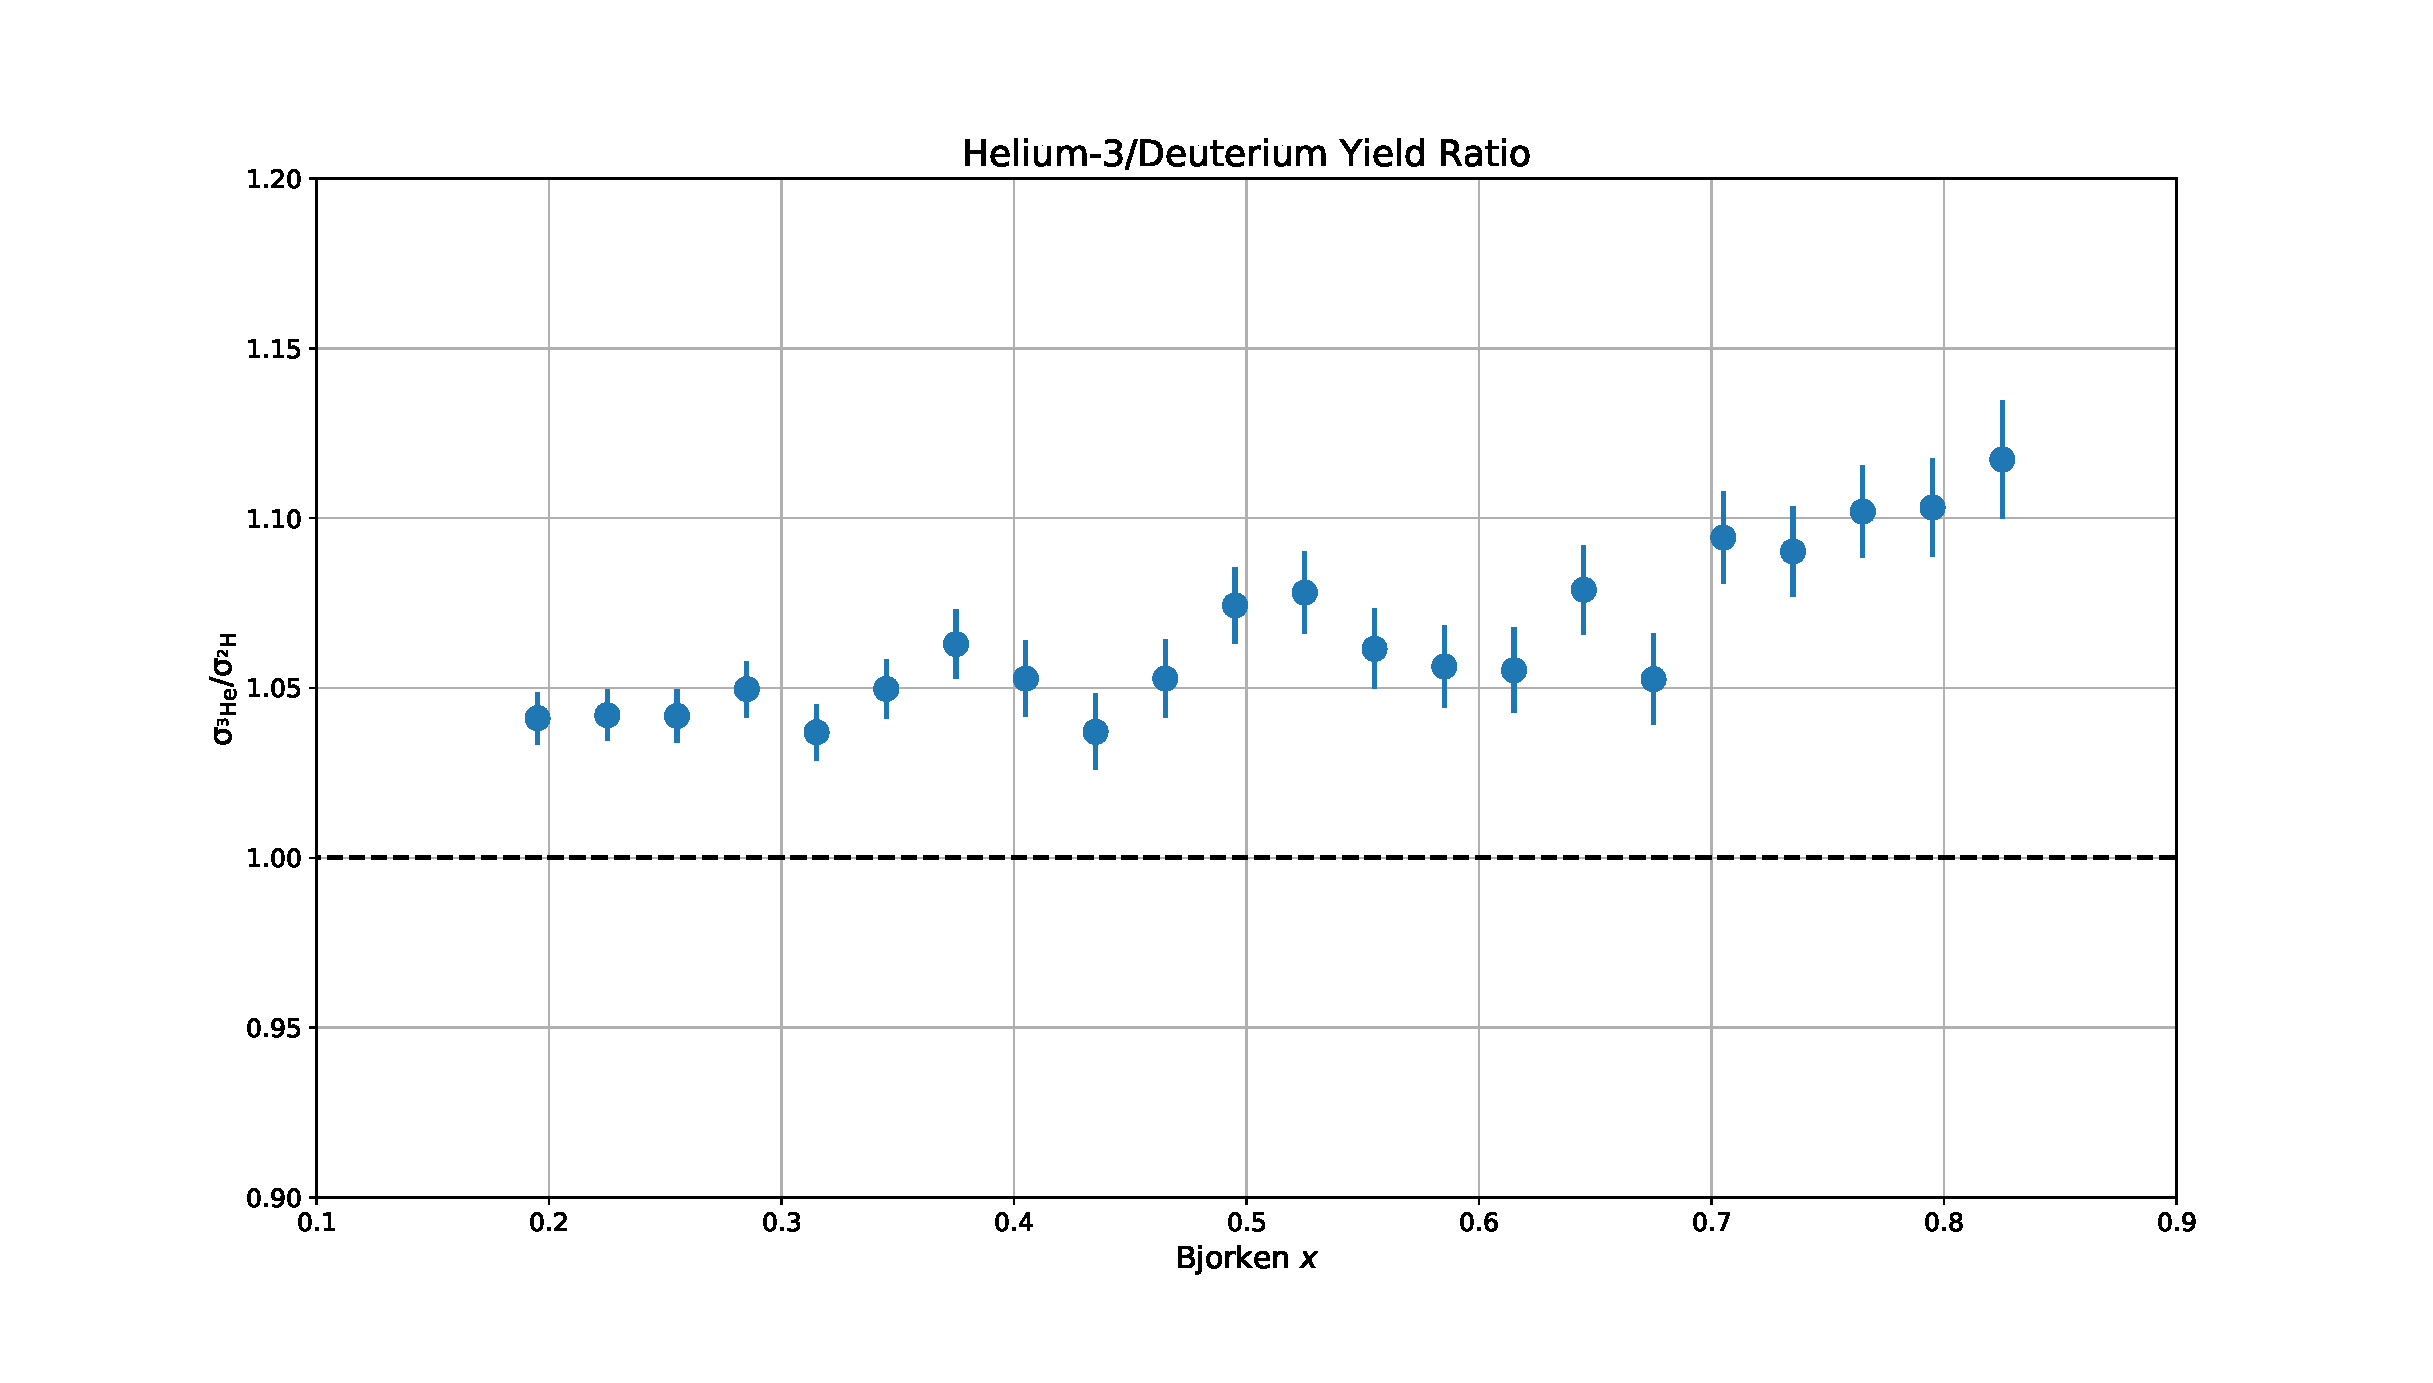
\includegraphics[width=\textwidth]{./results/fig/yield_ratio.eps}
	\caption{This plot shows the yield ratio of Helium-3/Deuterium.}
	\label{fig:yr1}
\end{figure}

\begin{table}
\center
\begin{tabular}{|c|c|c|c|c|}\hline
$x$ & $F_2^{^3\text{He}}/F_2^{^2\text{H}}$ & Statistical Uncertainty & Systematic Uncertainty & Radiative Corrections\\\hline\hline
\csvreader[late after line=\\\hline]{./results/tbl/no_norm.csv}{BinCenter=\x,Ratio=\ratio,RStat=\stat,RSyst=\syst, RC=\rc}{\x & \ratio & \stat & \syst & \rc}
\end{tabular}
\caption{Helium-3/Deuterium yield ratio. All systematic uncertainties discussed in Chapter \ref{chap:analysis}, except for that associated with the isoscalar correction, are included here.}
\label{tbl:fy1}
\end{table}

\section{Isoscalar Helium-3 EMC Yield Ratio}

The Helium-3 EMC ratio is the Helium-3/Deuterium ratio with Helium-3 corrected for proton-excess. That is, Helium-3 is transformed into a hypothetical isoscalar A=$\nicefrac{3}{2}$ nucleus. The isoscalar correction is done using the method described in Section \ref{sec:isocor}. This analysis uses an input of an $F_2^n/F_2^p$ fit of the extraction from the $^3$H/$^3$He MARATHON data. This data in shown in Figure \ref{fig:emc1} and listed in Table \ref{tbl:emc1}. The uncertainties plotted consist of statistical and all systematic uncertainties.

\begin{figure}[p]
	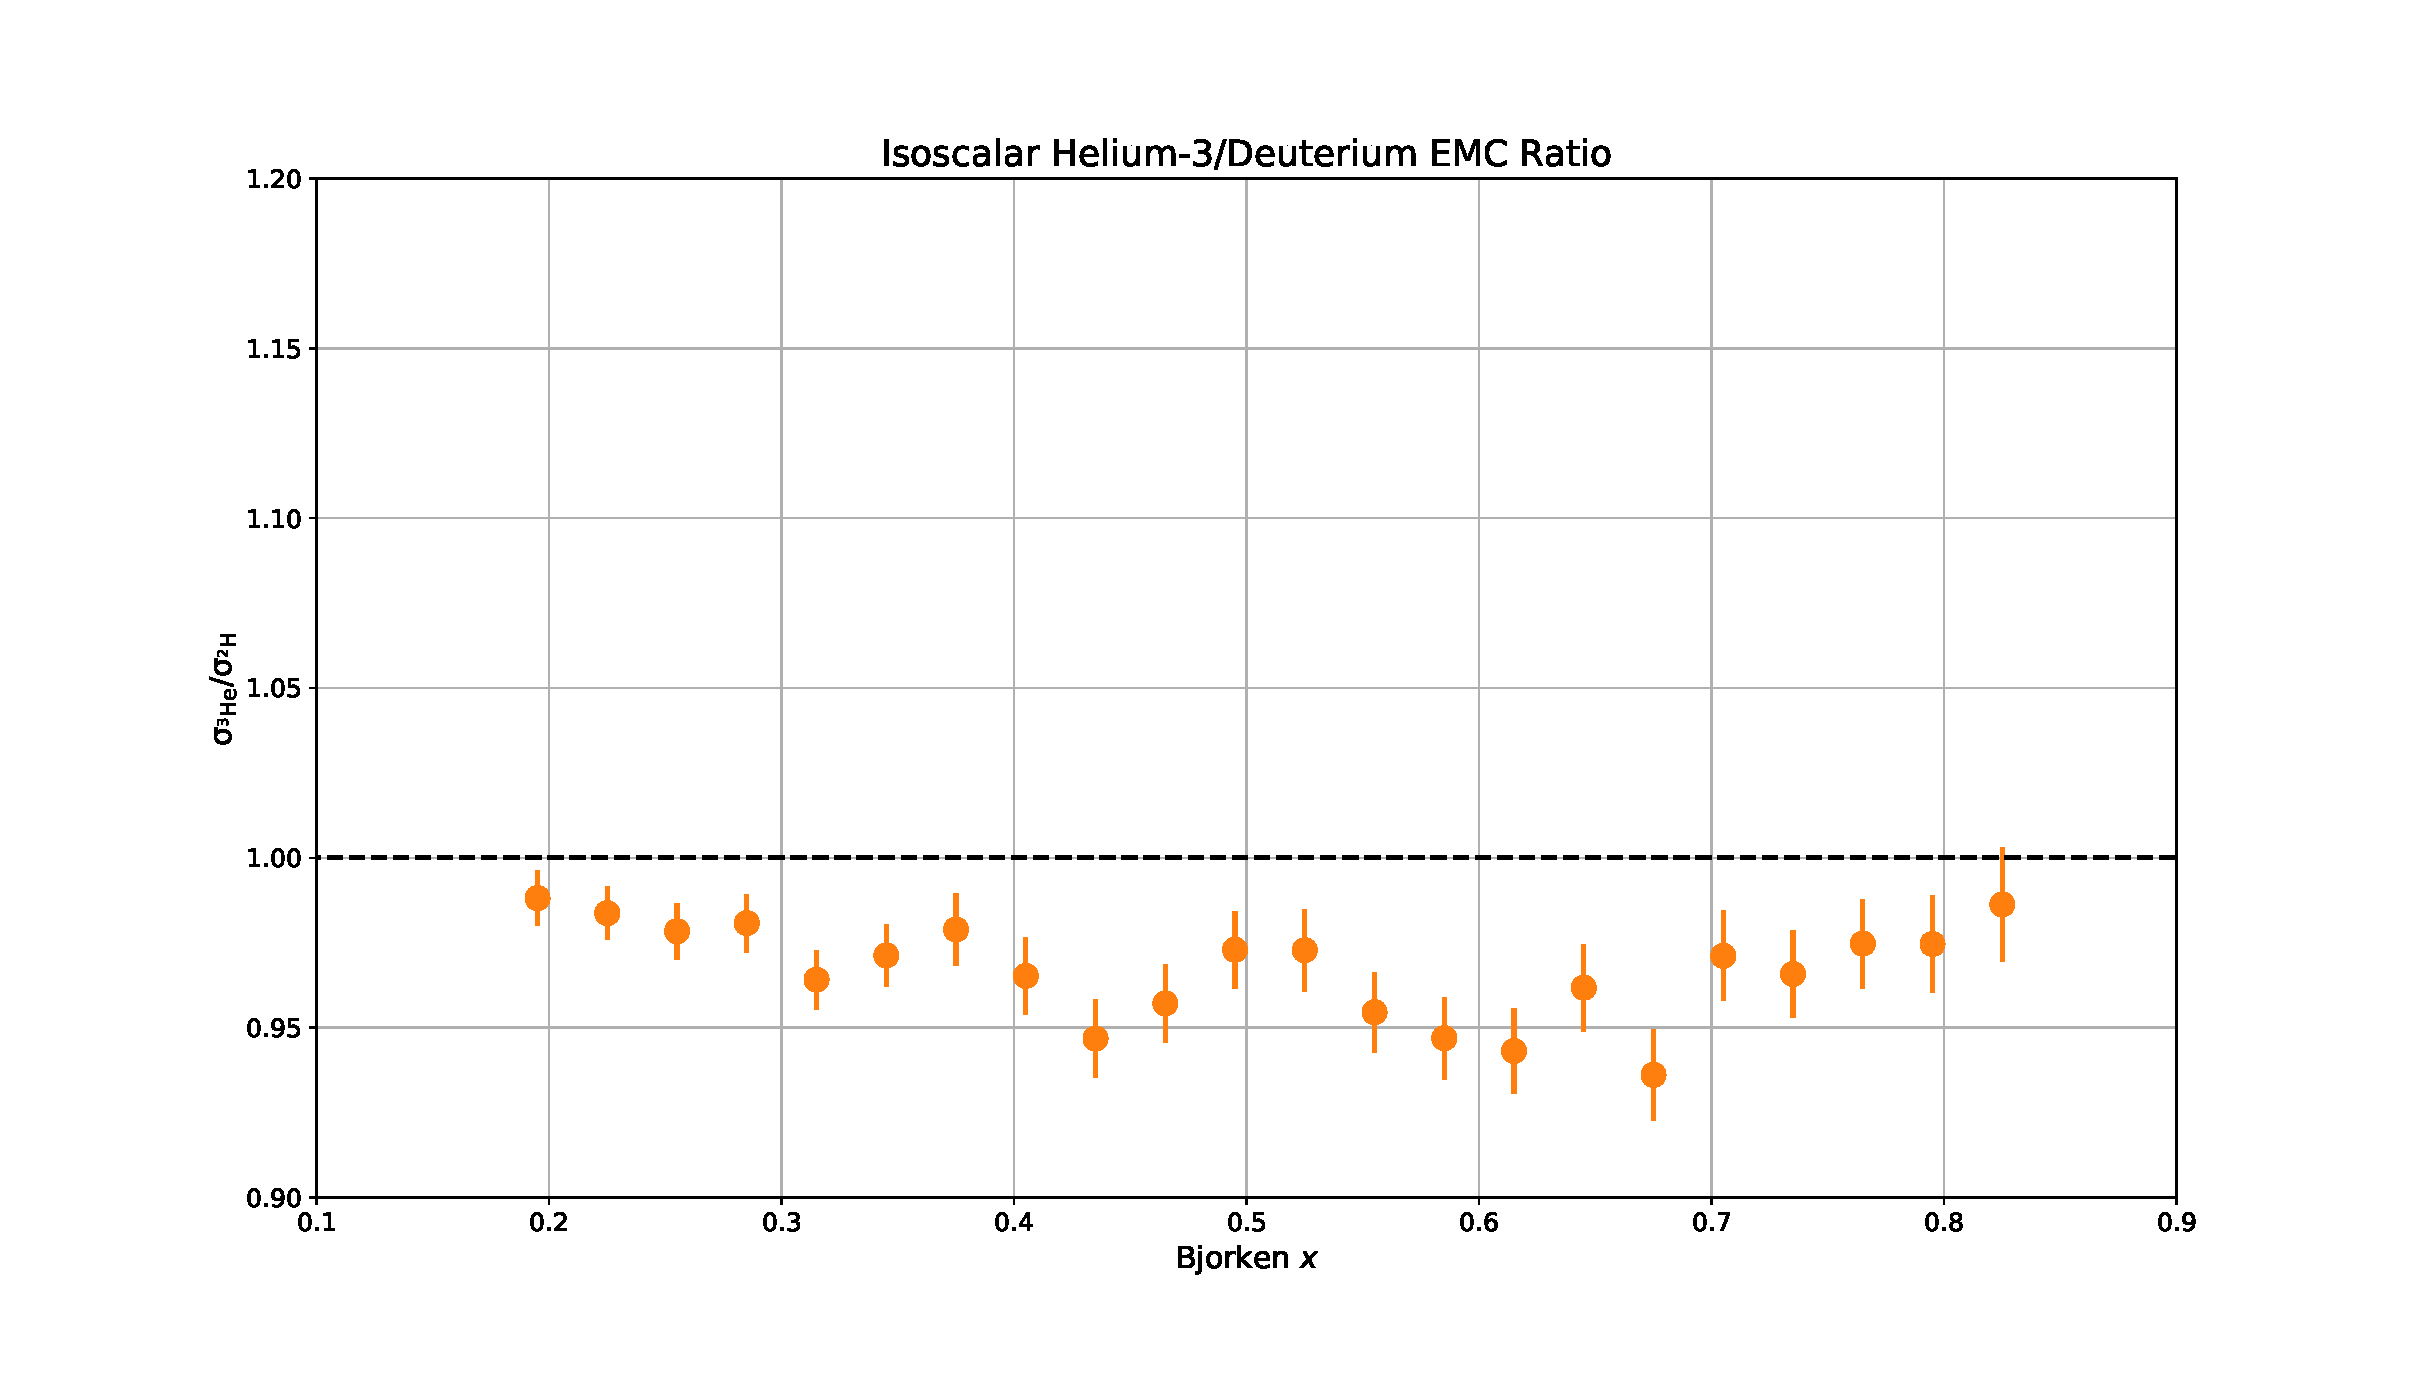
\includegraphics[width=\textwidth]{./results/fig/emc_ratio.eps}
	\caption{This plot shows the isoscalar EMC yield ratio of Helium-3.}
	\label{fig:emc1}
\end{figure}

\begin{table}
\center
\begin{tabular}{|c|c|c|}\hline
$x$ & Isoscalar Helium-3 EMC Ratio & Isoscalar Correction\\\hline\hline
\csvreader[late after line=\\\hline]{./results/tbl/no_norm.csv}{BinCenter=\x,Isoscalar_Ratio=\ratio,IsoRatio_Error=\err,IsoCor=\iso,IsoCorErr=\isoerr,RC=\rc}{\x & \ratio \ $\pm$ \err & \iso \ $\pm$ \isoerr}
\end{tabular}
\caption{Isoscalar Helium-3 EMC yield ratio. The listed uncertainty includes all systematic errors discussed in Chapter \ref{chap:analysis}, including the isoscalar correction uncertainty. The fractional contribution of the statistical uncertainty to this ratio is equivalent to the fractional contribution of the statistical uncertainty listed in Table \ref{tbl:fy1}.}
\label{tbl:emc1}
\end{table}

\section{Normalizing the data}

A feature of all EMC data is a unity crossing near $x=0.3$. This leads to the understanding that there are minimal nuclear effects in the region near $x=0.3$. A look at Figure \ref{fig:emc1} will show that this feature is not present in this data. An interpretation of this, as this work will examine, is that the Helium-3 data is in need of normalization. This is further justified when reading Reference \cite{Su_Thesis} in which it is noted that $^3$H/$^3$He required a $2.8\%$ normalization in order for the extraction of $F_2^n/F_2^p$ to agree with the extraction from $^2$H/$^1$H. The $^2$H/$^1$H data is in agreement with world data. This method is derived from and described in Reference \cite{KP2010}.

The normalization for this data is determined in the same way that it was determined for the $^3$H/$^3$He data. This is done by first extracting $F_2^n/F_2^p$ from the Helium-3/Deuterium Yield Ratio using the method described in Section \ref{sec:F2ratio}. Since nuclear effects are minimal near $x=0.3$, it is expected that all $F_2^n/F_2^p$ extractions should agree in this region. Figure \ref{fig:f2r} shows that, without normalization, this is not the case.

\begin{figure}[p]
	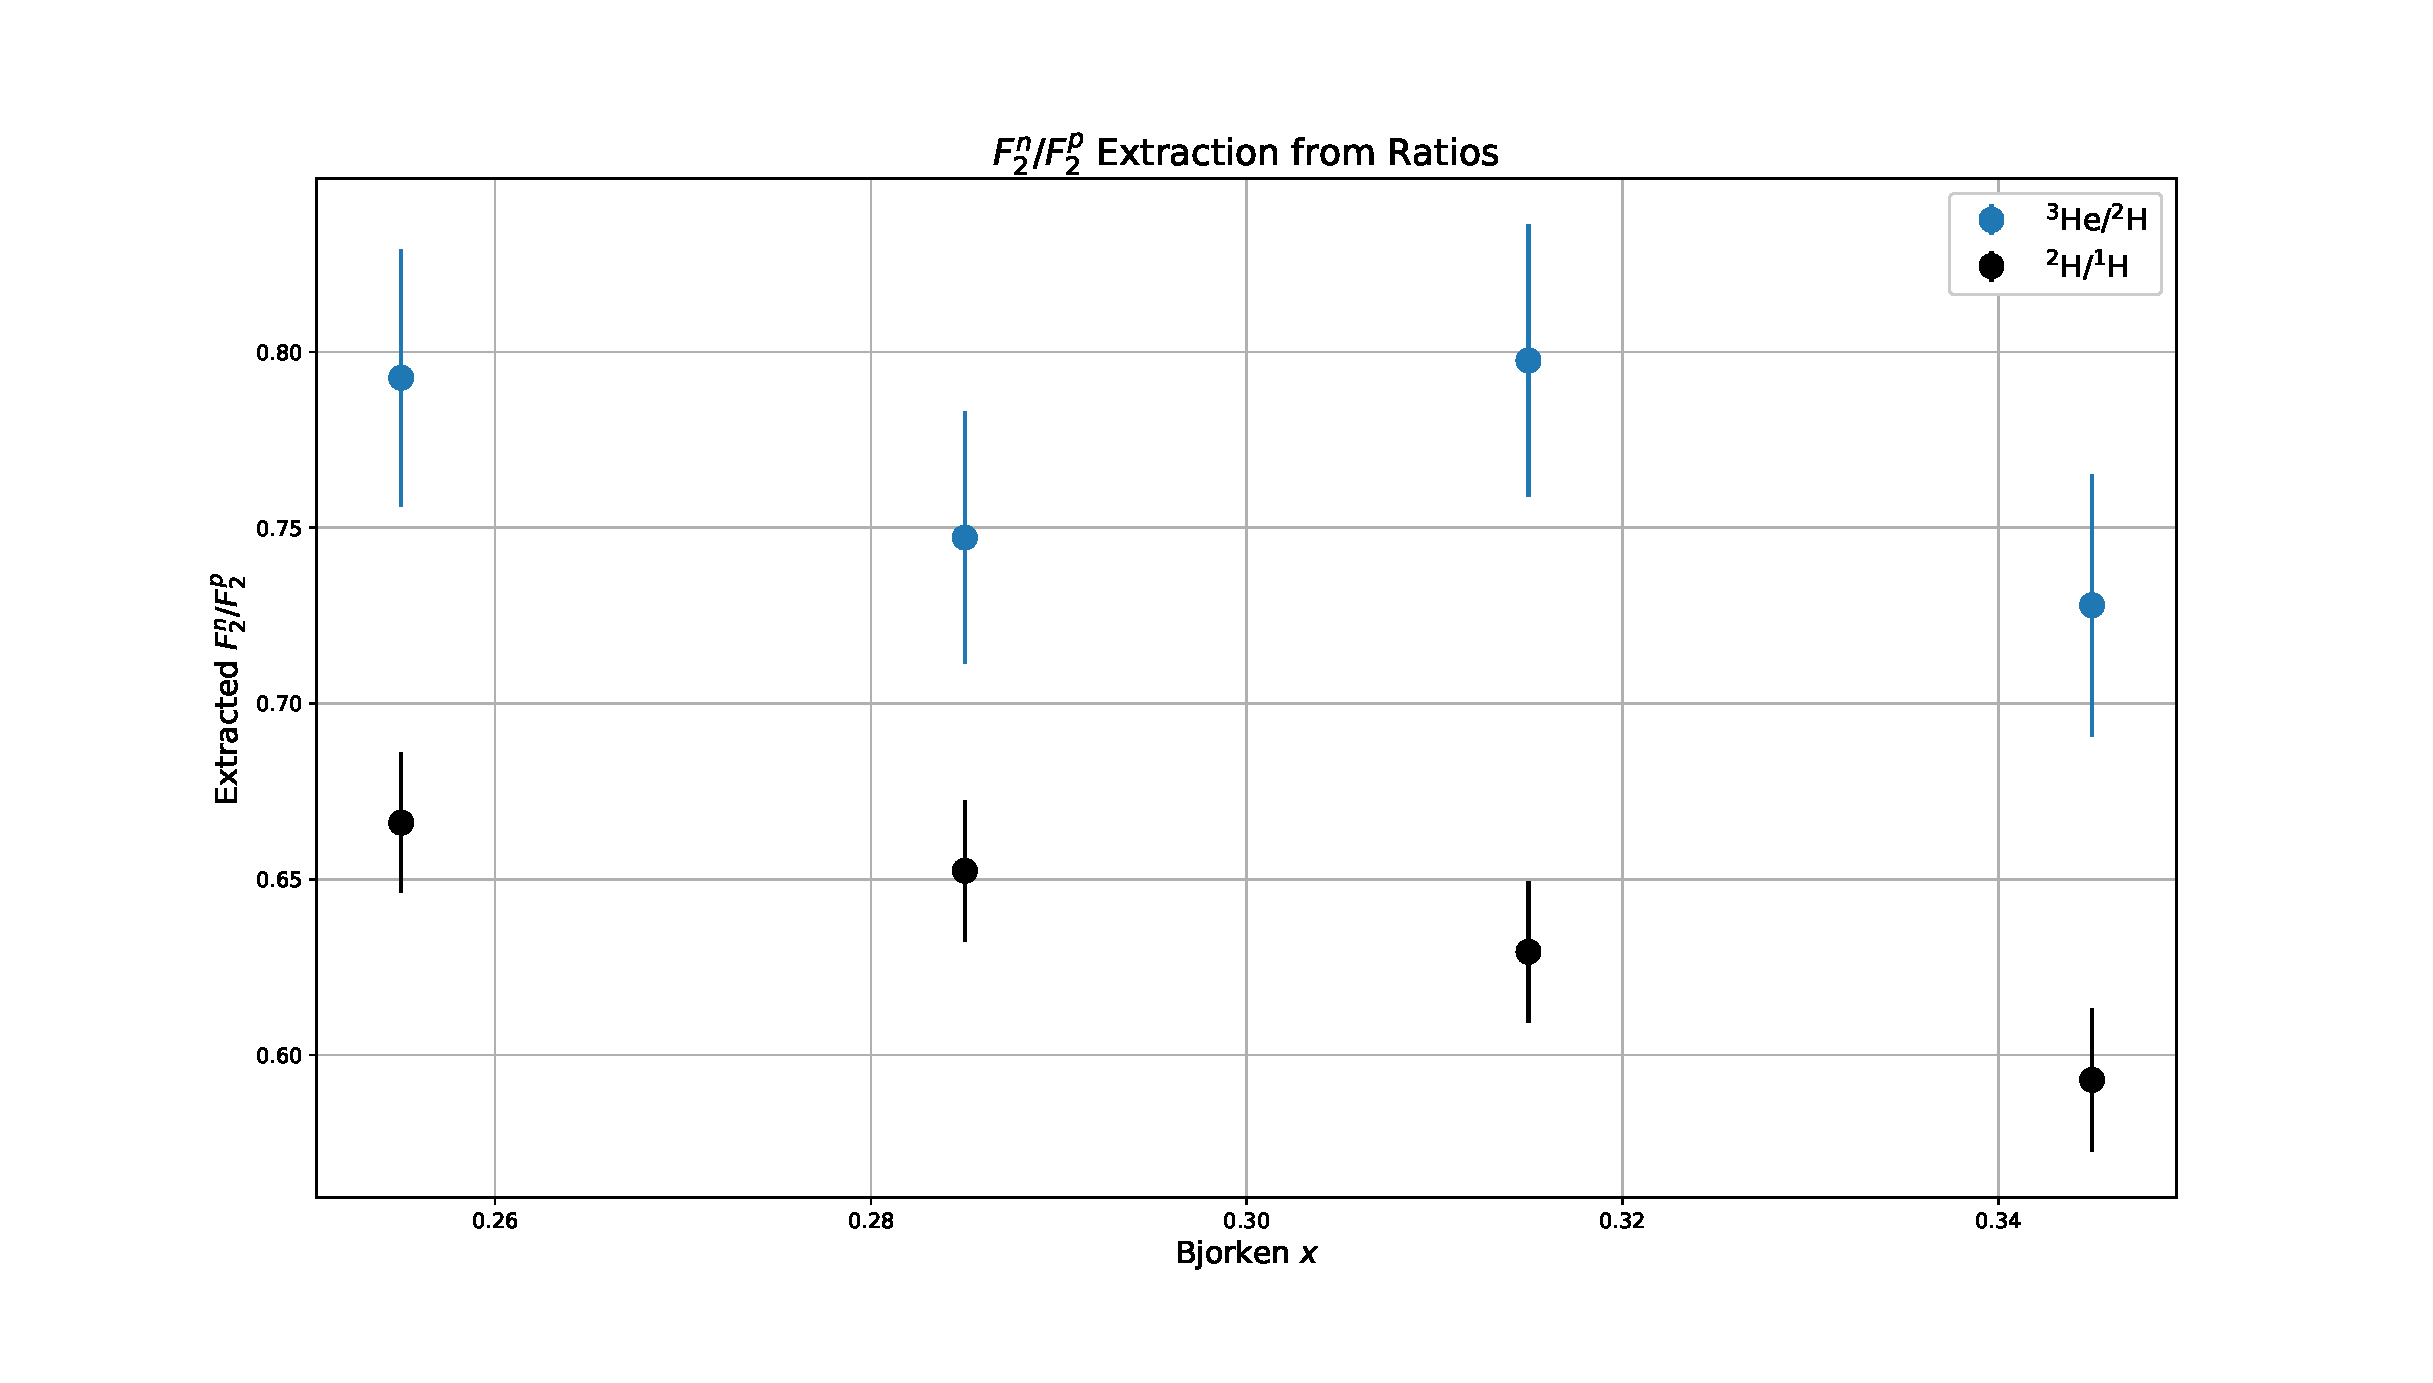
\includegraphics[width=\textwidth]{./results/fig/f2r.eps}
	\caption{$F_2^n/F_2^p$ extracted from the Helium-3/Deuterium yield ratio compared to the extraction from the MARATHON Deuterium/Hydrogen data.}
	\label{fig:f2r}
\end{figure}

This extraction requires a model input. For this analysis, the Kulagin-Petti (KP) model is used. This model was chosen by comparing it to the non-isoscalar yield ratio. Of the models examined, this one best matched the overall shape of the data. A comparison of the Helium-3/Deuterium yield ratio with the KP model prediction is shown in Figure \ref{fig:KP_comp}.

\begin{figure}[p]
	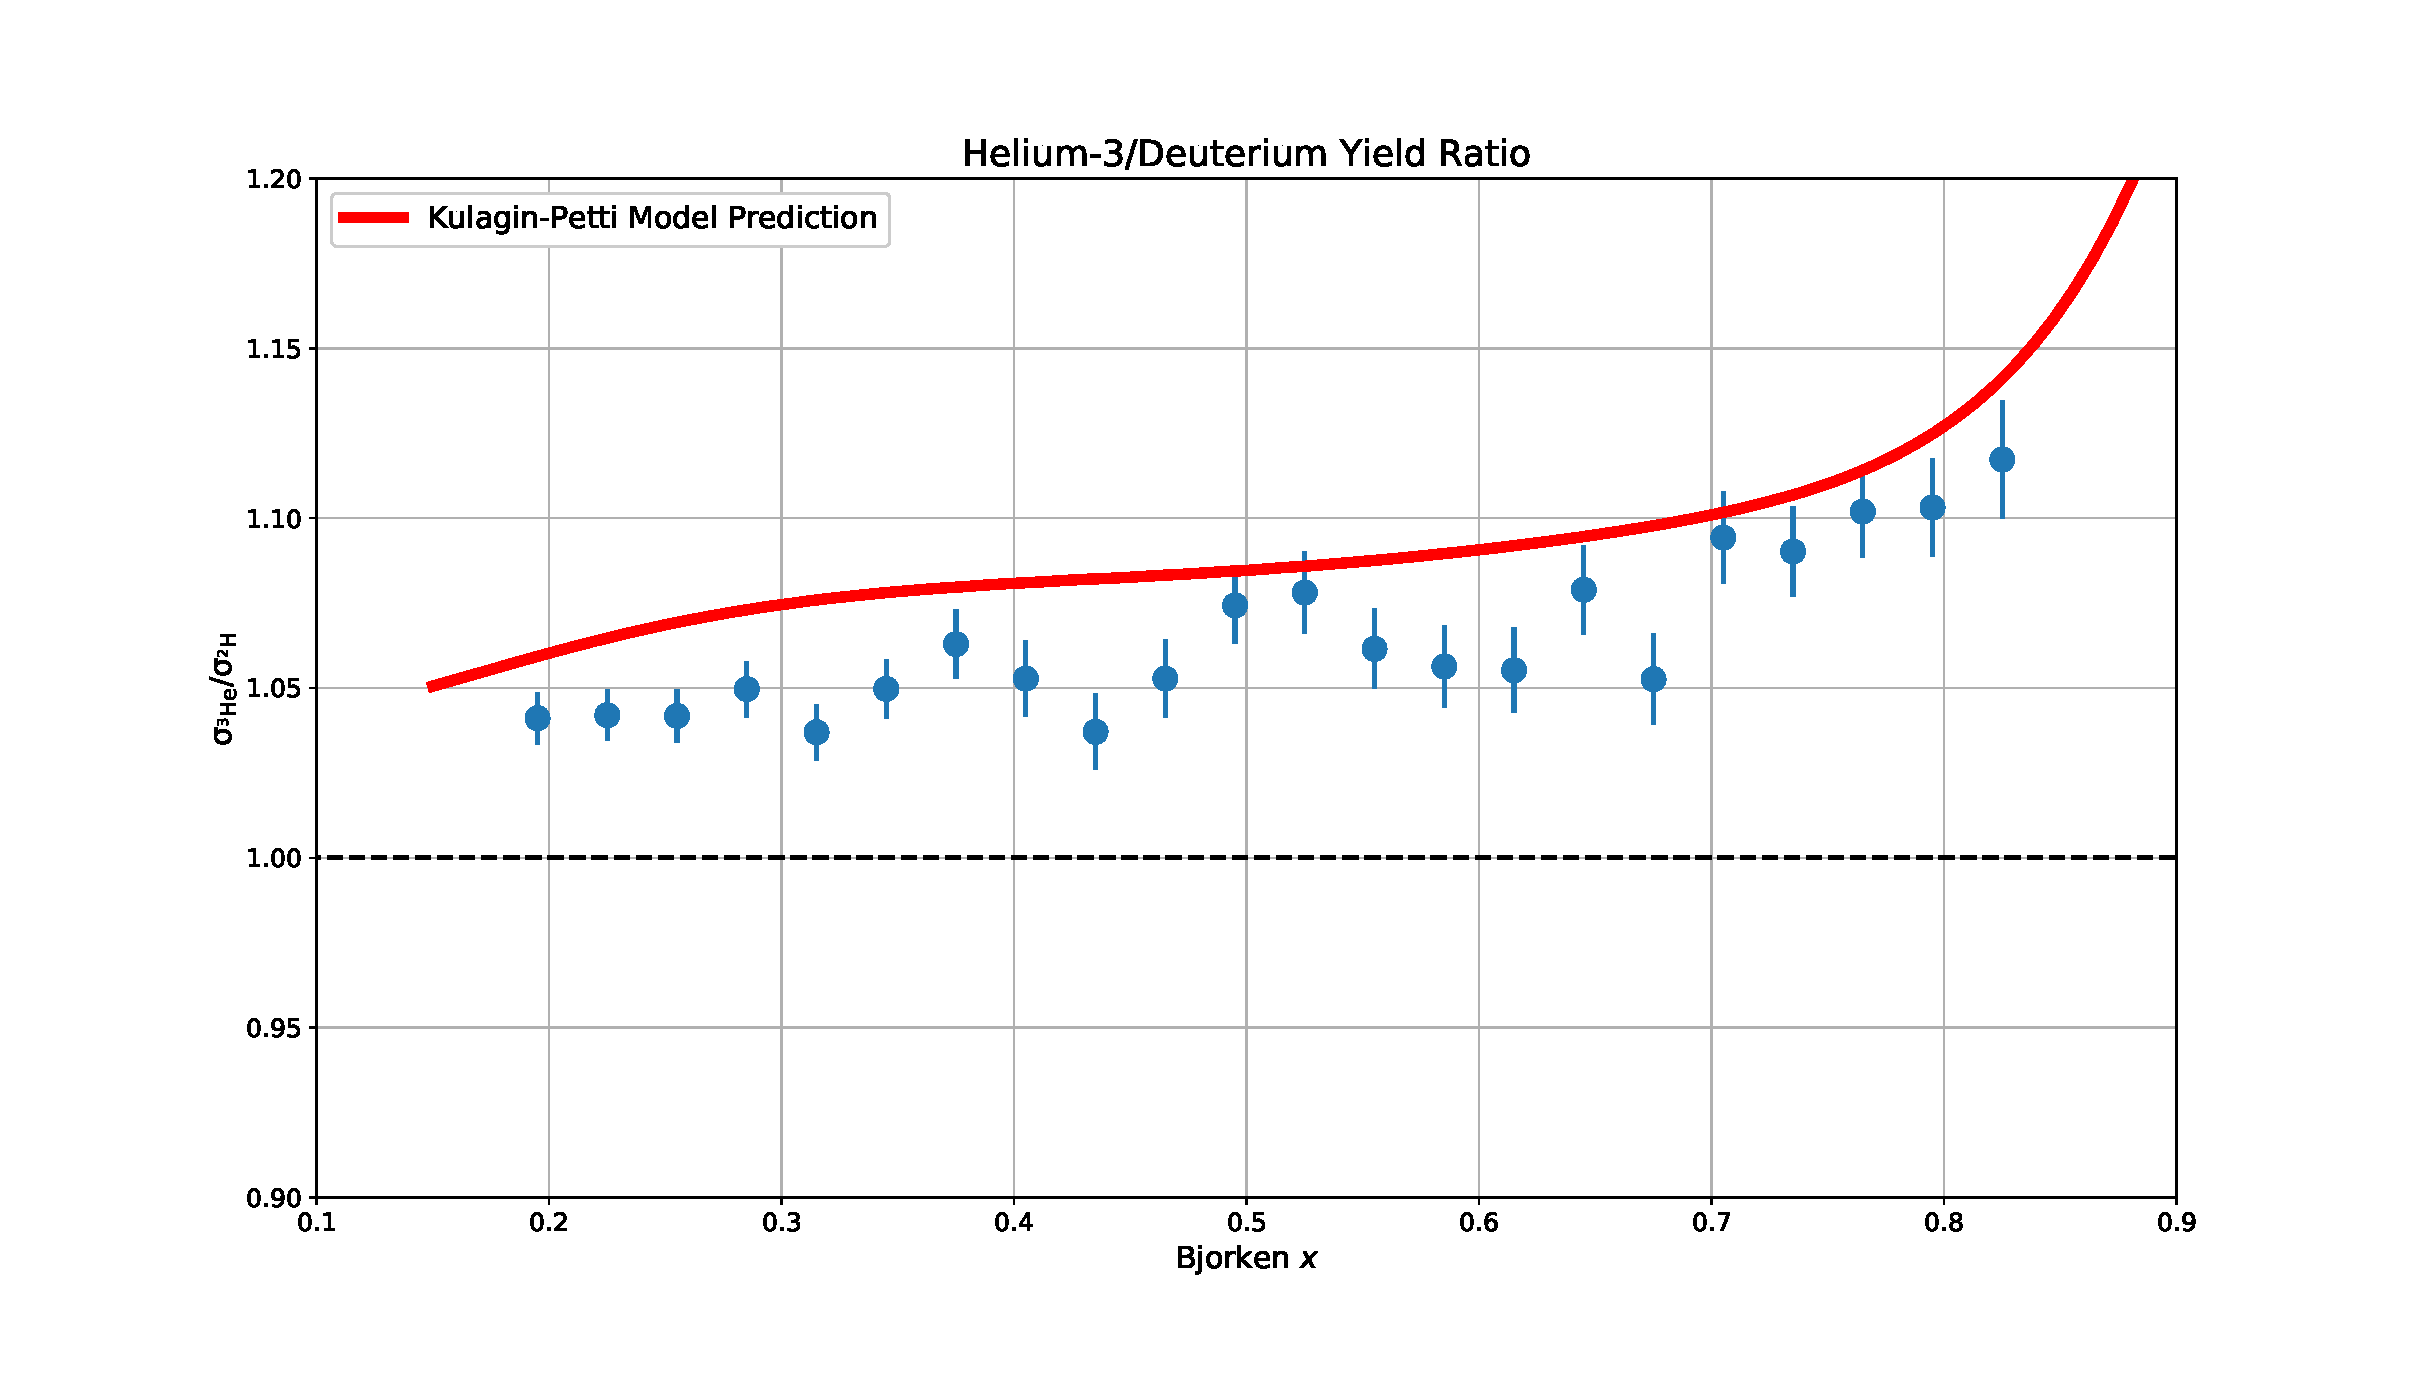
\includegraphics[width=\textwidth]{./results/fig/KPcomp.eps}
	\caption{Helium-3/Deuterium yield ratio compared to the KP model. While the data does not match in value, it does match in shape.}
	\label{fig:KP_comp}
\end{figure}

The normalization is determined by calculating the reduced $\chi^2$ of the four data points symmetric around $x=0.3$ ($x=0.255$, $0.285$, $0.315$, and $0.345$) when compared to the extraction of $F_2^n/F_2^p$ from $^2$H/$^1$H. This process takes into account the variance, $\sigma^2$, of the $^3$He/$^2$H data in order to minimize the effect of statistical fluctuations. Different normalizations of the yield ratio are iterated over in steps of $0.1\%$. This is continued until the extractions are clearly deviating again and the normalization with the minimum reduced $\chi^2$ is chosen. For this data, a normalization of $2.8\%$ is found to be necessary for the $F_2^n/F_2^p$ extraction to match that of $^2$H/$^1$H. Figure \ref{fig:f2r_norm} shows the $F_2^n/F_2^p$ extraction with this normalization applied. Figure \ref{fig:ratio_norm} shows the Helium-3/Deuterium yield ratio and isoscalar Helium-3 EMC ratio with this this normalization applied. Table \ref{tbl:ratio_norm} lists the data with the normalization applied.

\begin{figure}[p]
	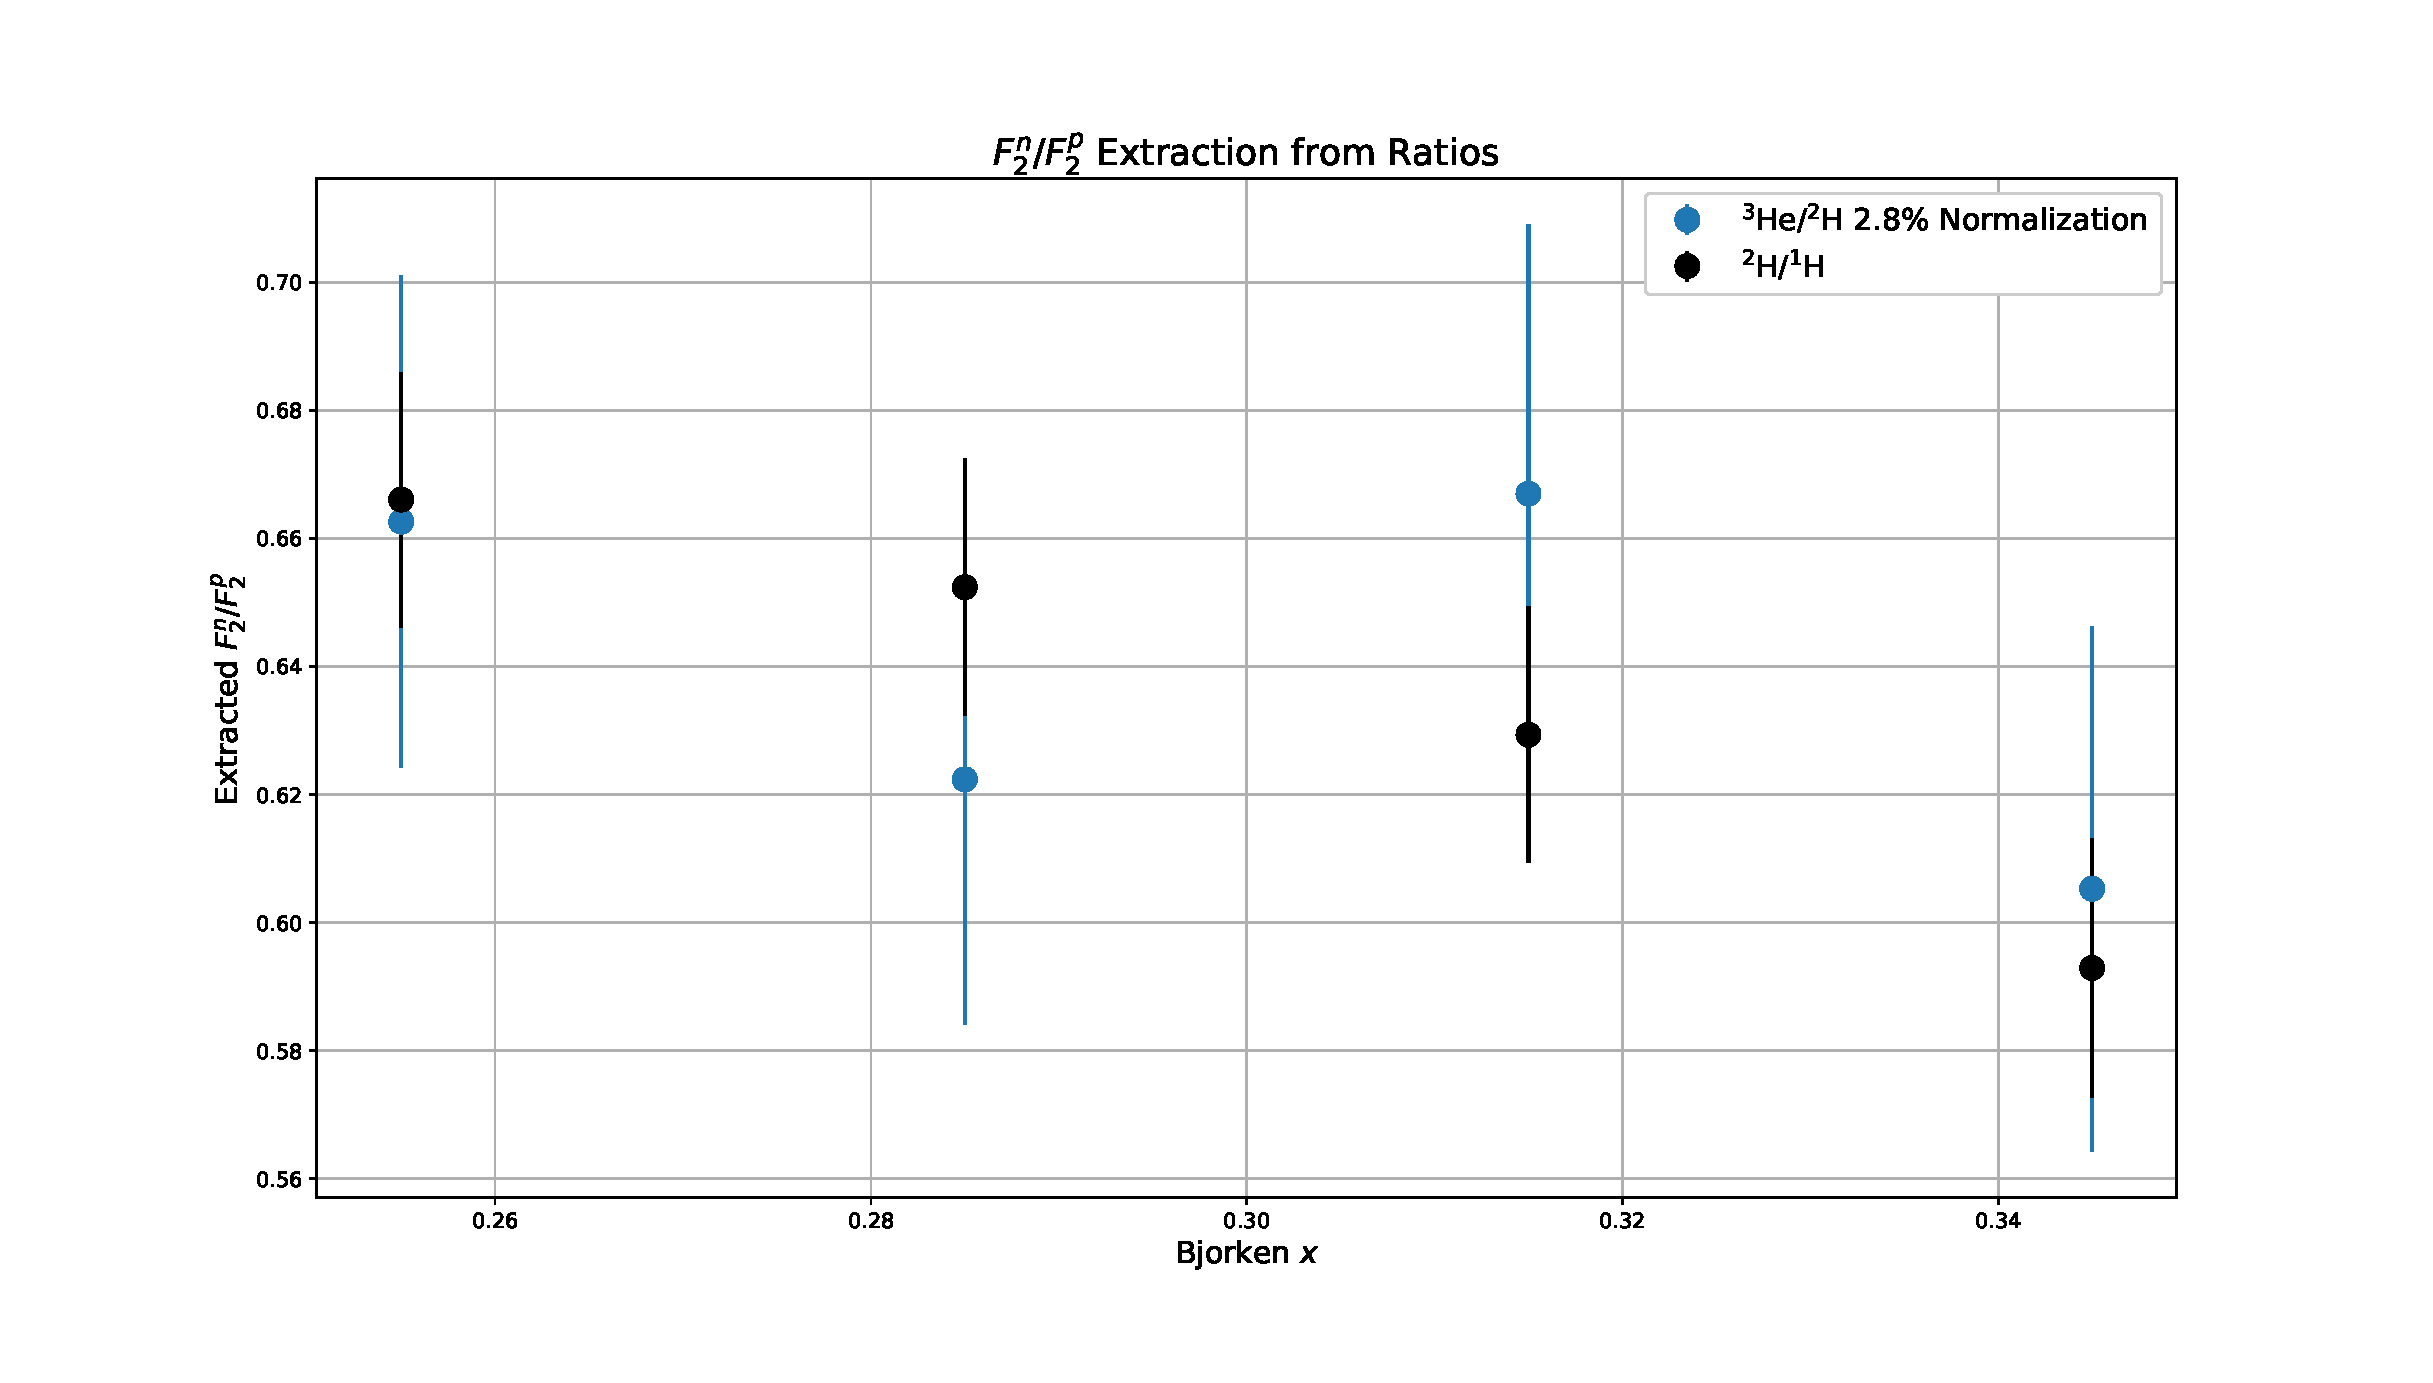
\includegraphics[width=\textwidth]{./results/fig/f2r_norm.eps}
	\caption{$F_2^n/F_2^p$ extracted from the Helium-3/Deuterium yield ratio, with a $2.8\%$ normalization, compared to the extraction from the MARATHON Deuterium/Hydrogen data.}
	\label{fig:f2r_norm}
\end{figure}

\begin{figure}[p]
	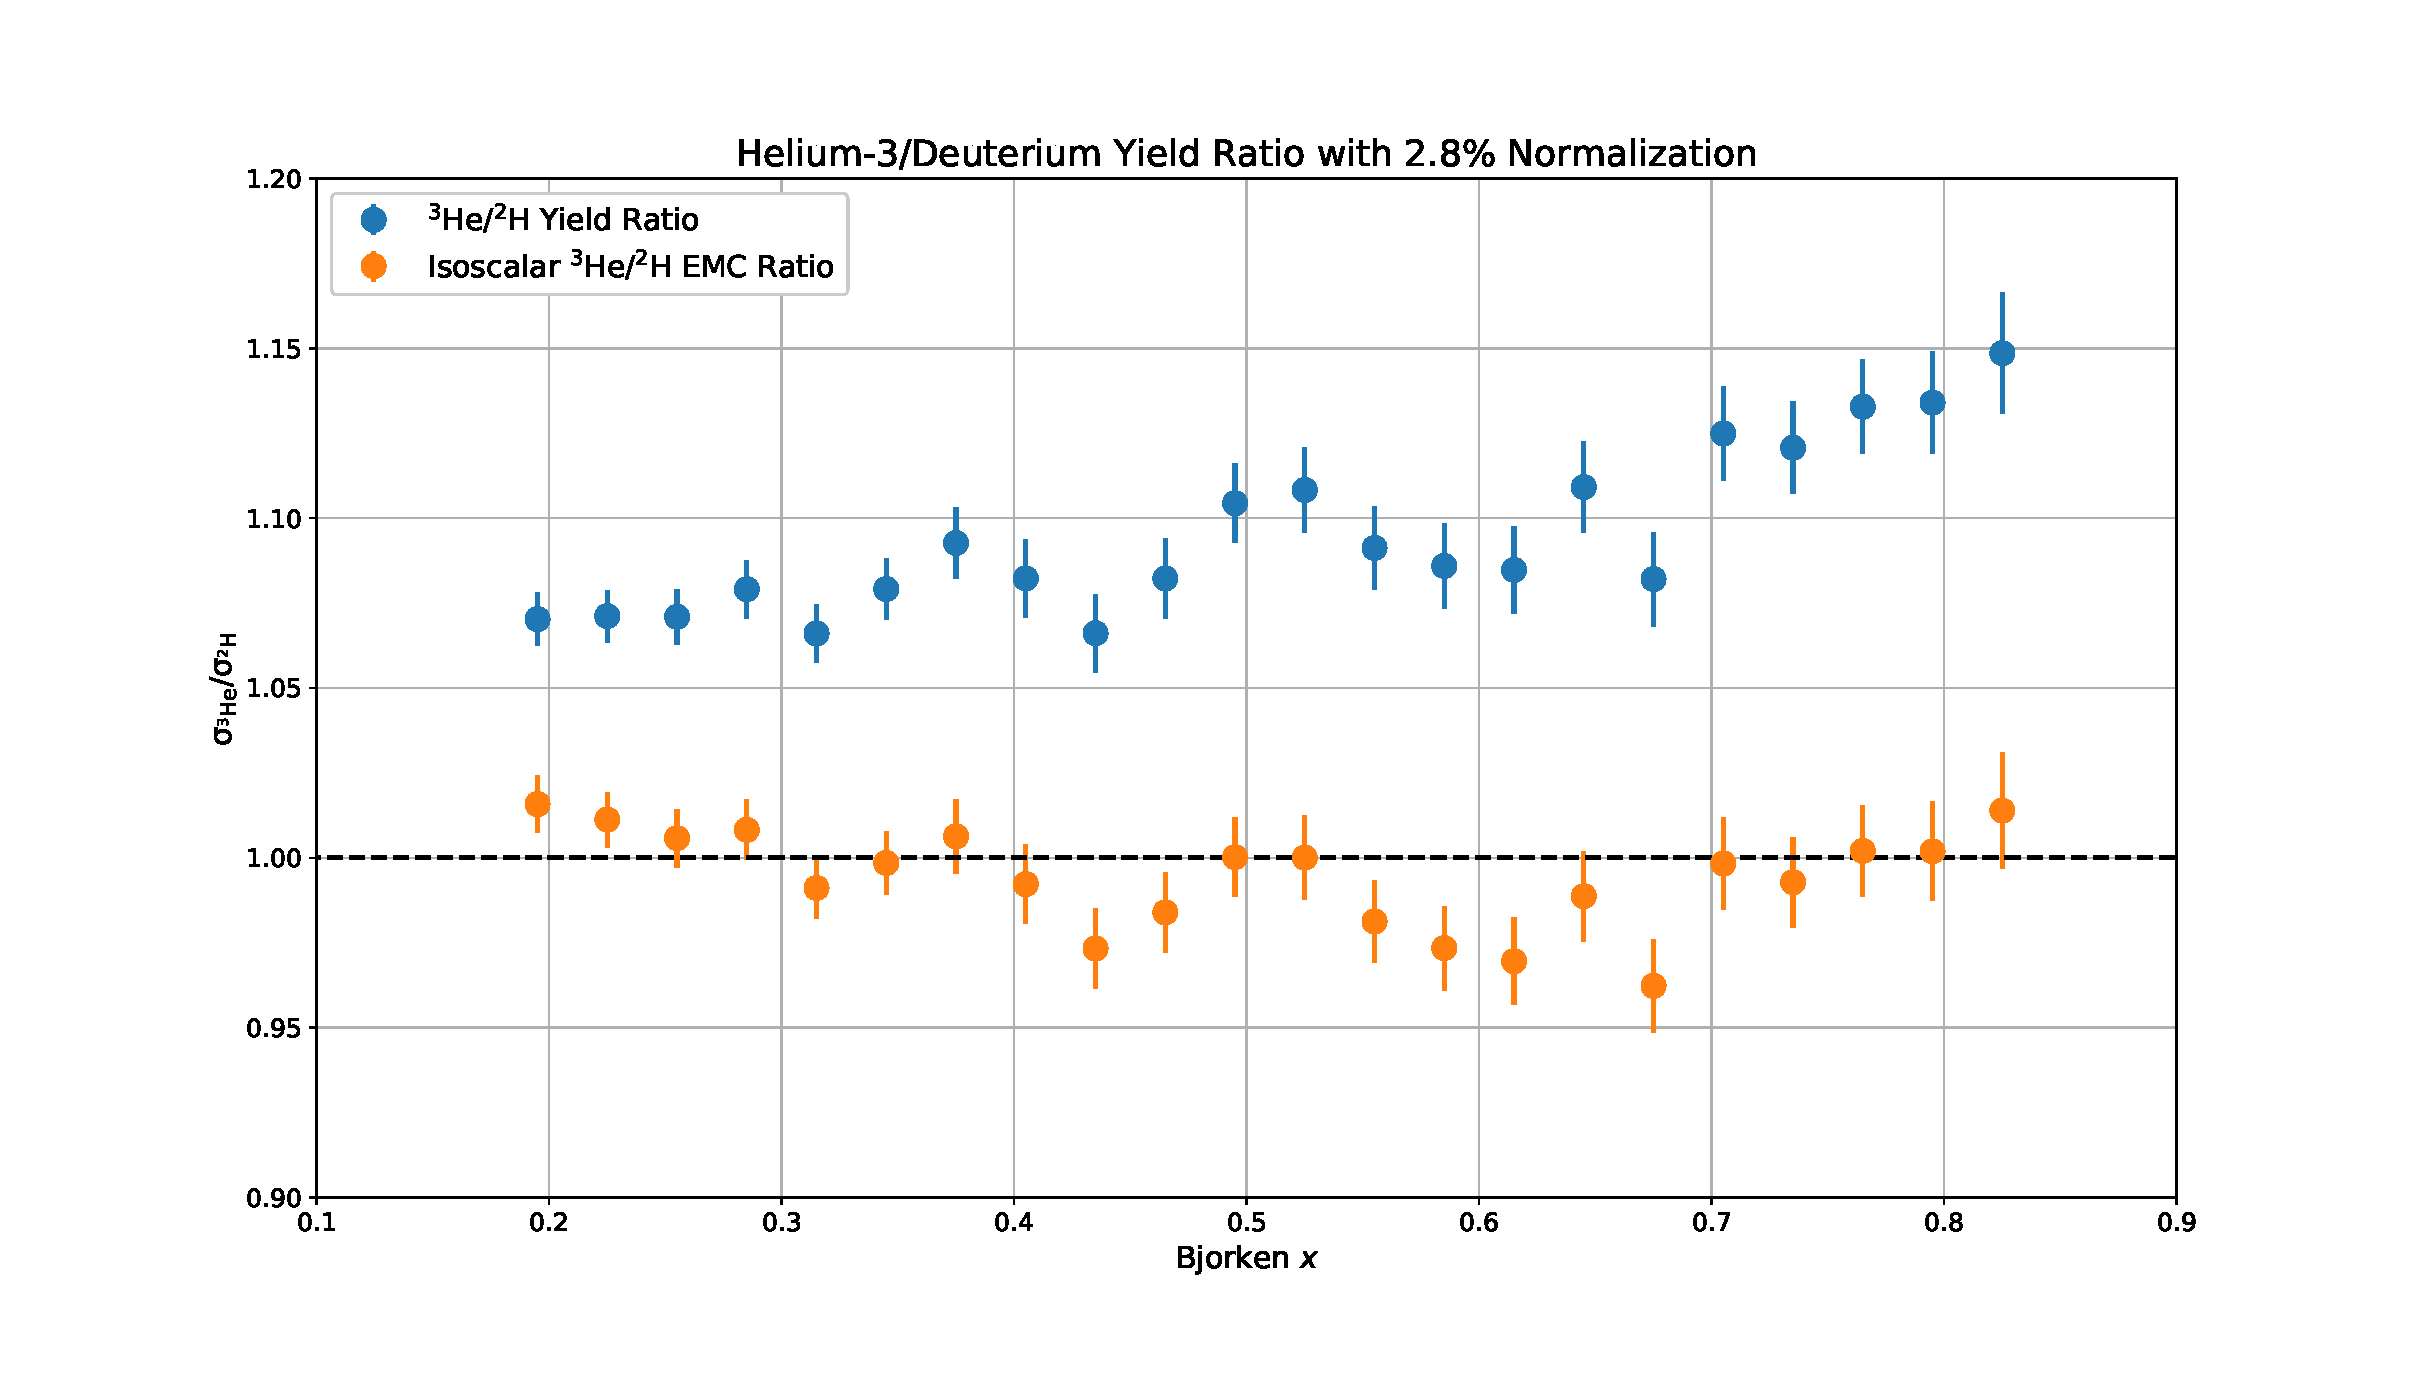
\includegraphics[width=\textwidth]{./results/fig/ratio_norm.eps}
	\caption{This plot shows the yield ratio of Helium-3/Deuterium and the isoscalar EMC yield ratio of Helium-3 with a $2.8\%$ normalization applied.}
	\label{fig:ratio_norm}
\end{figure}

\begin{table}
\center
\begin{tabular}{|c|c|c|}\hline
$x$ & Normalized $F_2^{^3\text{He}}/F_2^{^2\text{H}}$ & Normalized Isoscalar Helium-3 EMC Ratio \\\hline\hline
\csvreader[late after line=\\\hline]{./results/tbl/no_norm.csv}{BinCenter=\x,Ratio=\ratio,Ratio_Error=\err,Isoscalar_Ratio=\isoratio,IsoRatio_Error=\isoerr}{\x & \ratio \ $\pm$ \err & \isoratio \ $\pm$ \isoerr}
\end{tabular}
\caption{Helium-3/Deuterium yield ratio and Isoscalar Helium-3 EMC yield ratio with $2.8\%$ normalization applied. The listed uncertainties include all statistical and systematic uncertainties.}
\label{tbl:ratio_norm}
\end{table}

\section{Comparison to Previous Helium-3 EMC Data}

There are two previous measurements of the Helium-3 EMC ratio: HERMES \cite{hermes,hermes_errata} and JLab E03-103 \cite{e03103}. Figure \ref{fig:rawcomp} shows a comparison of the measured MARATHON yield ratio, without isoscalar corrections or normalization, to the non-isoscalar E03-103 and HERMES data. The HERMES data is only published corrected for proton-excess. The data in \cite{nmc_f2} was used to approximate the isoscalar correction applied in order to arrive at the non-isoscalar data. The HERMES data is published with a $0.9\%$ normalization from comparison to SLAC and NMC $^4$He data, which is removed for the following comparisons, except where explicitly stated. These three sets of data agree well within error bars, with the HERMES data having a slightly higher offset. The offset of the HERMES data is within normalization uncertainty.

\begin{figure}[p]
	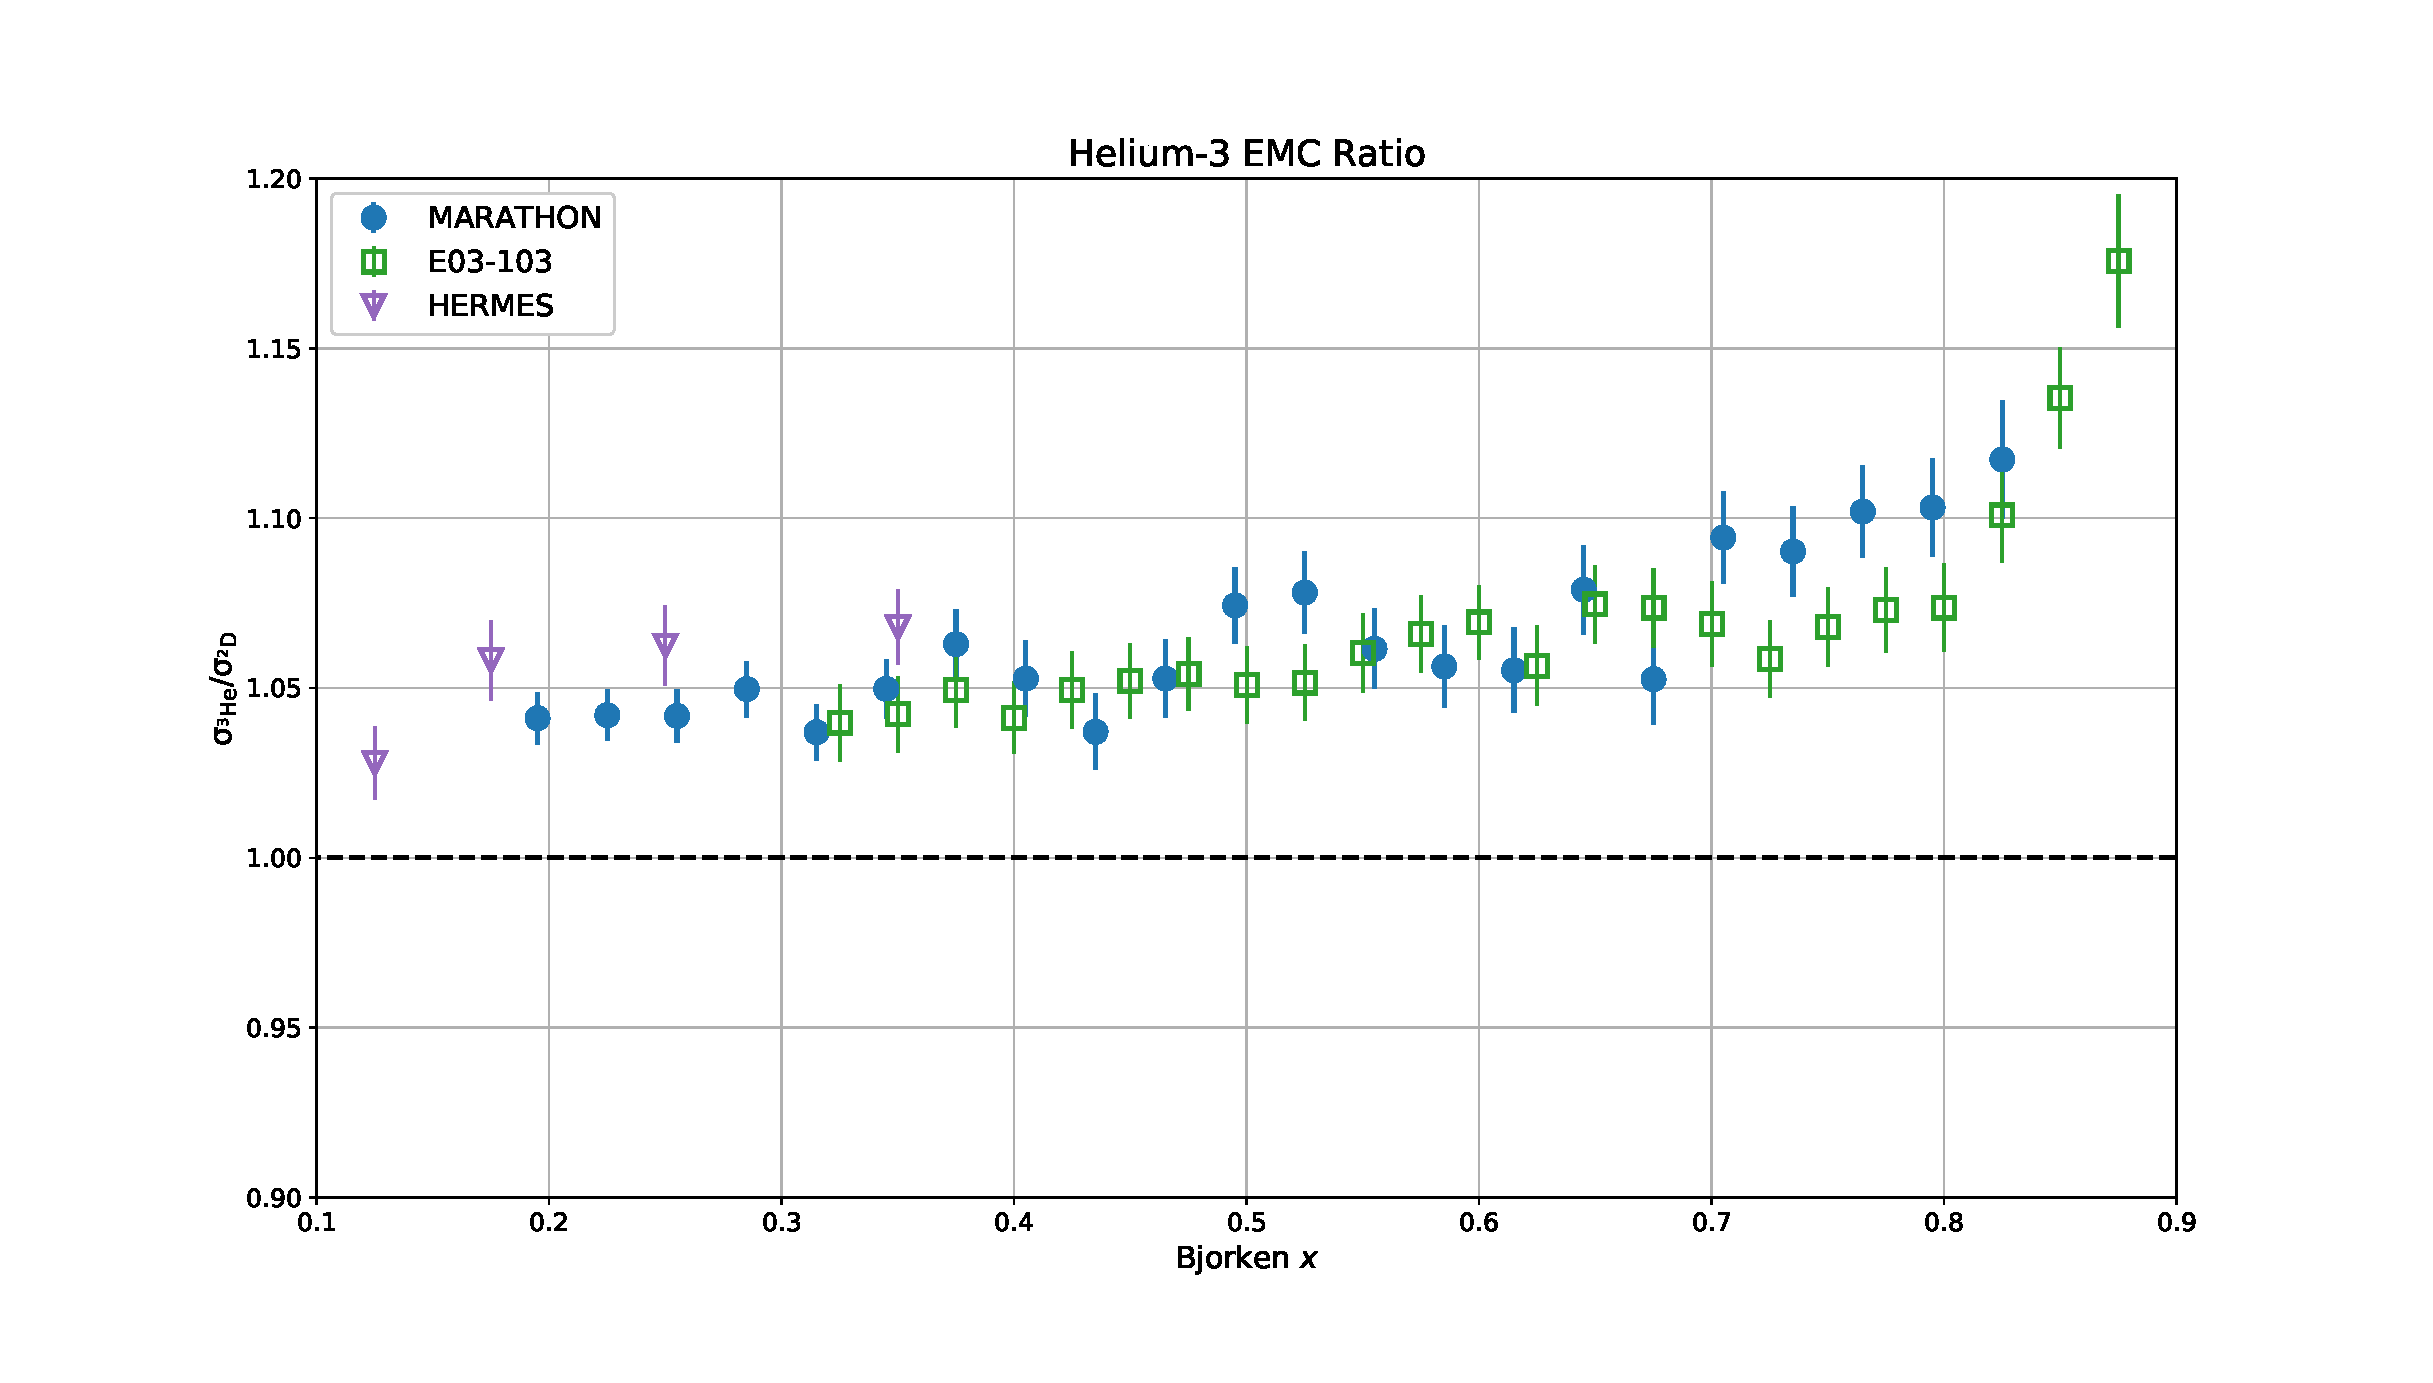
\includegraphics[width=\textwidth]{./results/fig/rawcomp.eps}
	\caption{A comparison of non-isoscalar, unnormalized data from MARATHON, E03-103, and HERMES.}
	\label{fig:rawcomp}
\end{figure}

Each of these three measurements has had a different isoscalar correction applied. Figure \ref{fig:isocomp} shows these three sets of data, each with the isoscalar correction from their original analysis applied. This figure does not have any normalizations applied. This figure again shows good data agreement and a slight offset of the HERMES data, which is within normalization uncertainty.

\begin{figure}[p]
	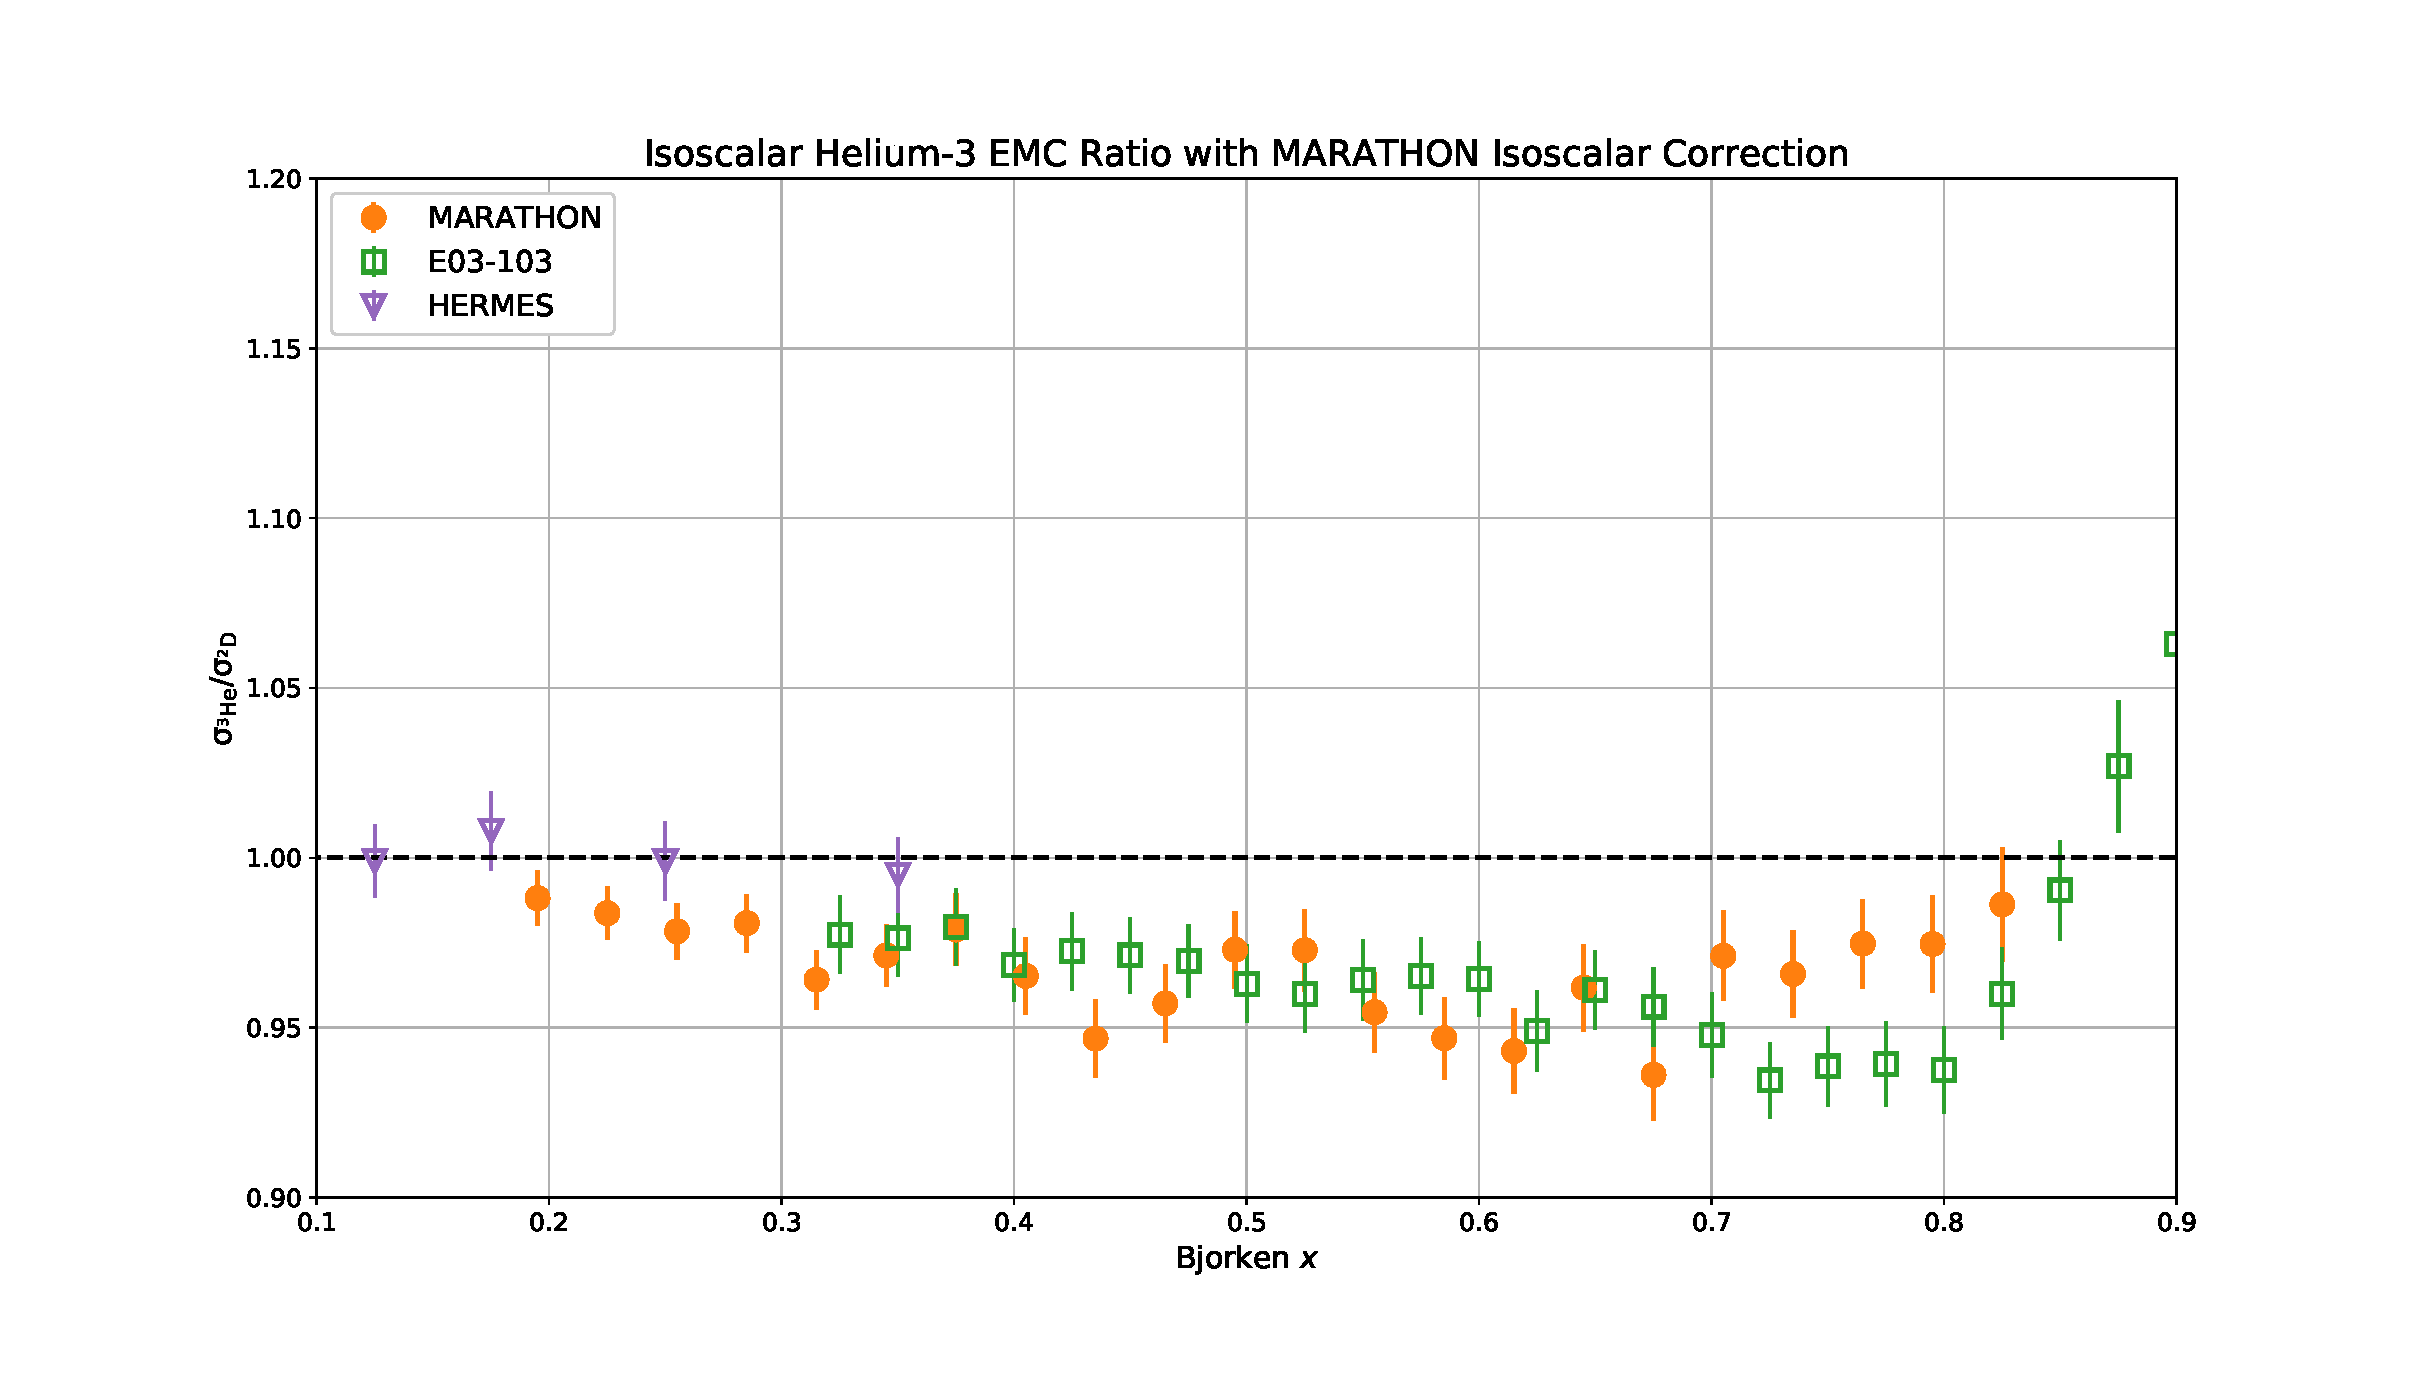
\includegraphics[width=\textwidth]{./results/fig/iso_comp.eps}
	\caption{A comparison of isoscalar, unnormalized data from MARATHON, E03-103, and HERMES. The isoscalar corrections applied are the corrections determined by each experiment.}
	\label{fig:isocomp}
\end{figure}

For a more direct comparison, it is useful to apply the same isoscalar correction to all data. As the non-isoscalar HERMES data is unpublished, the HERMES data is shown with their determined isoscalar correction. Figure \ref{fig:maraisocomp} shows these data sets with the MARATHON isoscalar correction applied. Given the clear agreement between MARATHON and E03-103 data, any normalization applied to one must be applied to the other. Figure \ref{fig:maraisonormcomp} shows the normalized isoscalar data with the MARATHON isoscalar correction and normalization also applied to the E03-103 data. In this figure, the HERMES normalization of $0.9\%$ is also applied. The culmination of these normalizations yields good agreement between all data sets and a disappearance of the offset in the HERMES data.

\begin{figure}[p]
	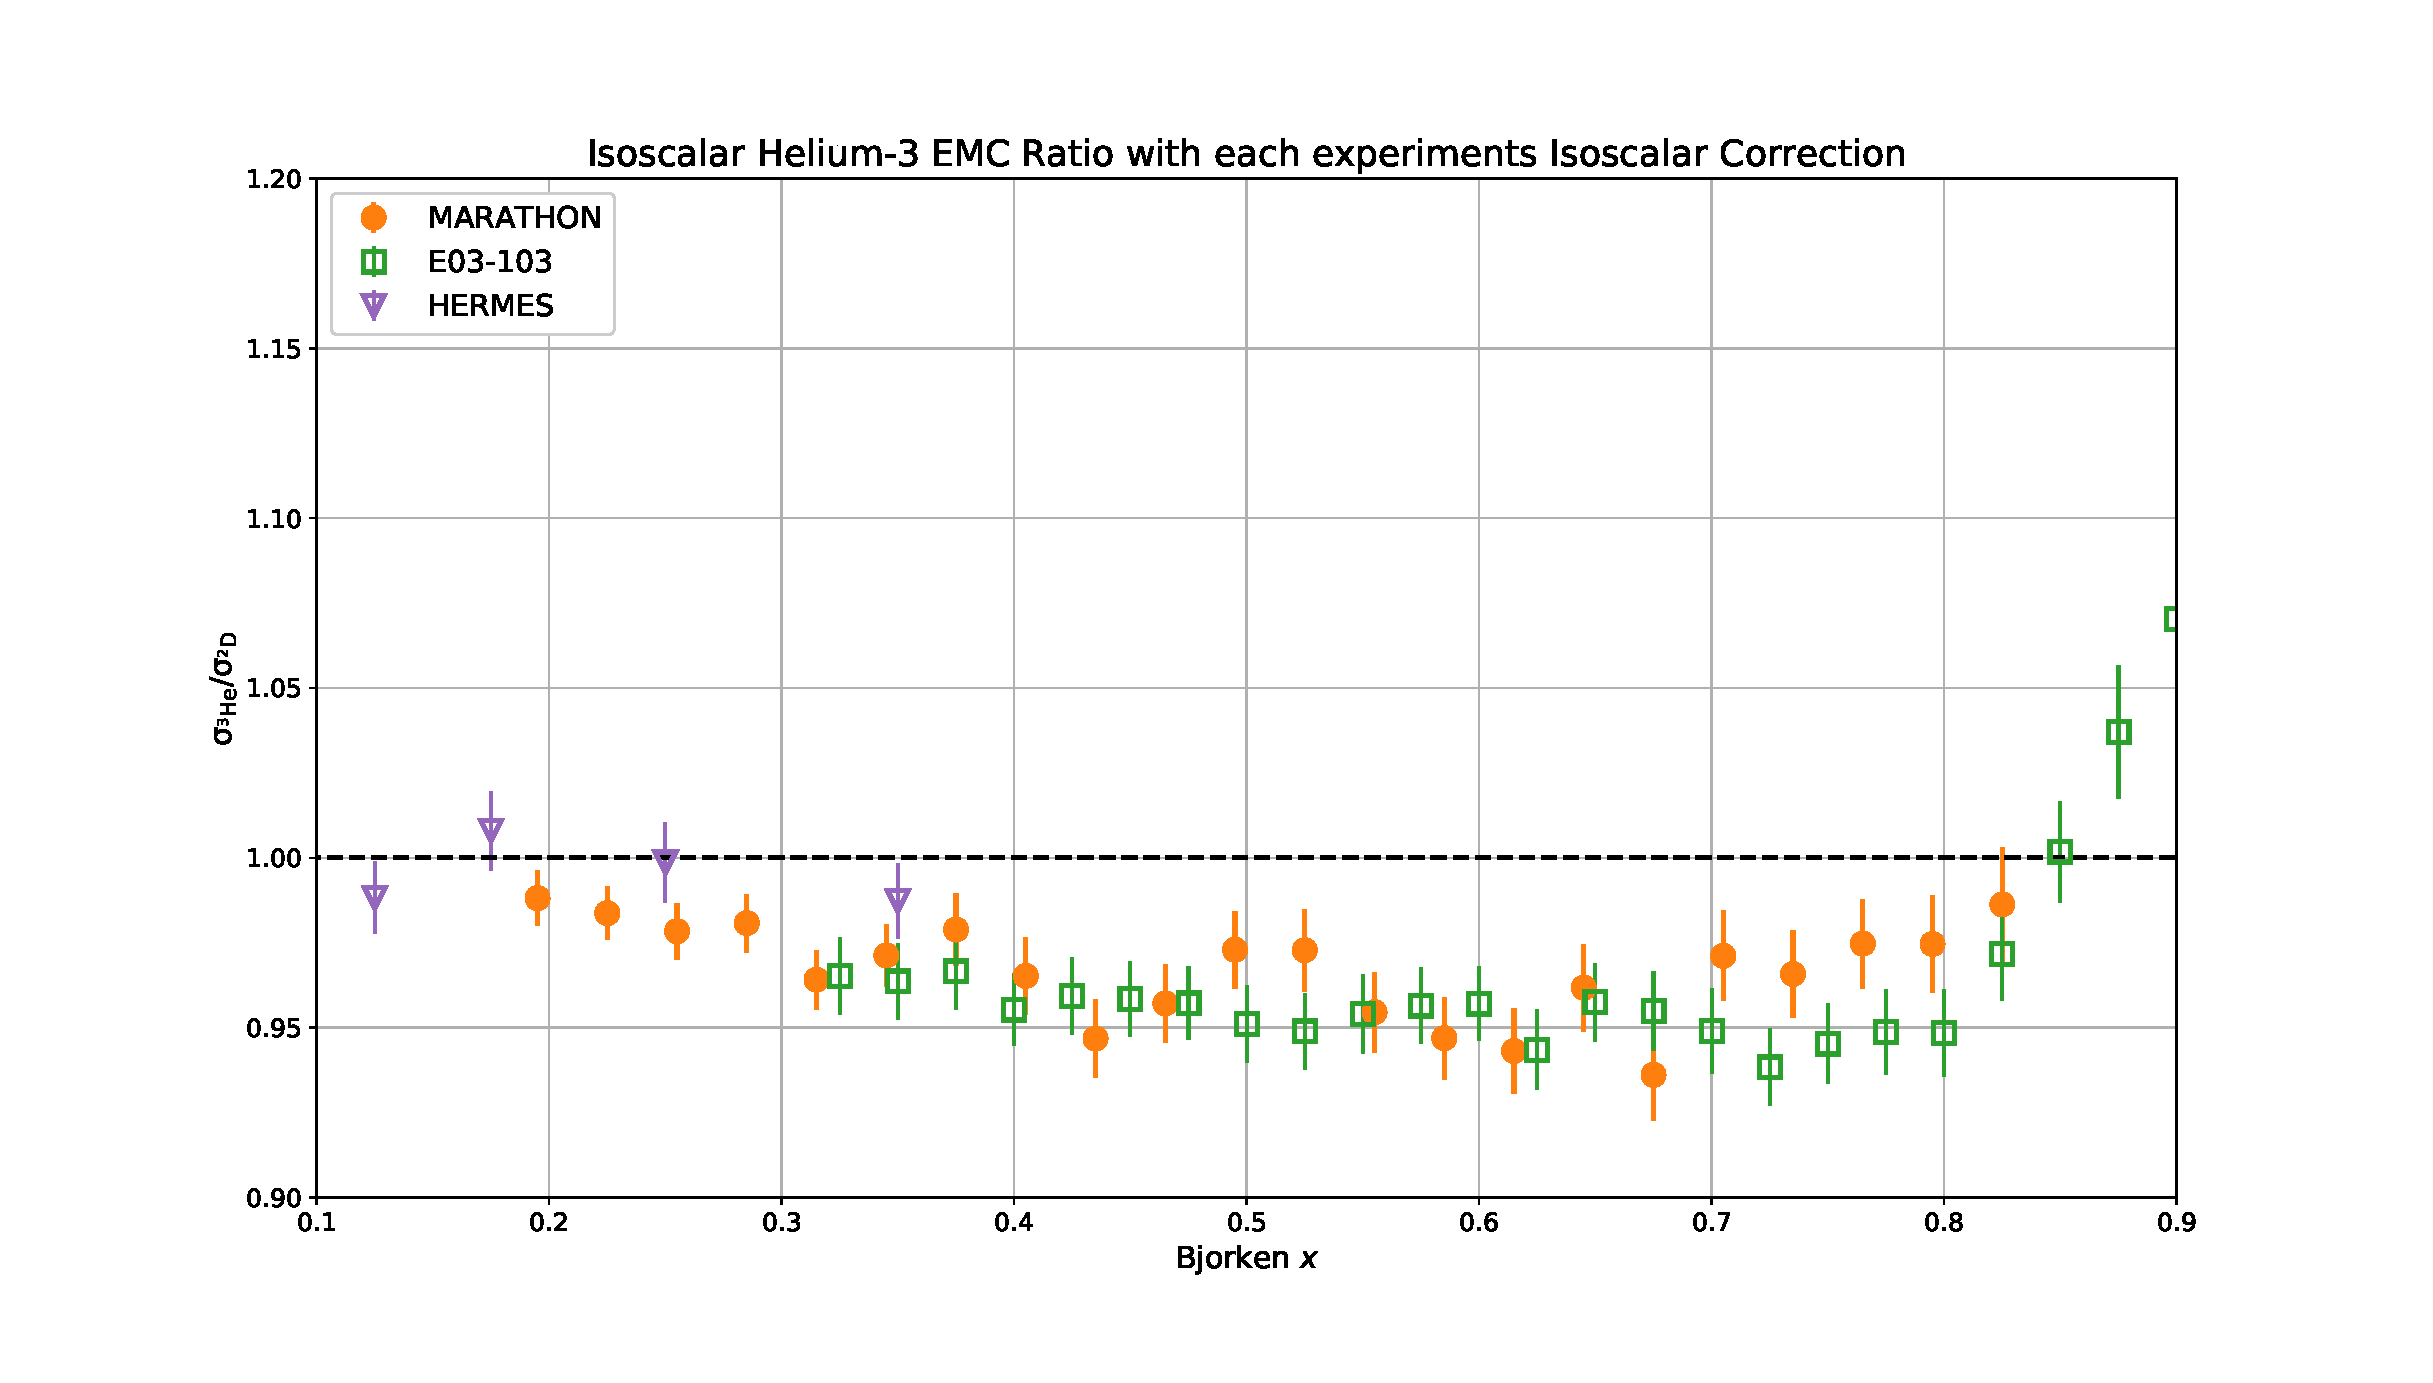
\includegraphics[width=\textwidth]{./results/fig/maraiso_comp.eps}
	\caption{A comparison of isoscalar, unnormalized data from MARATHON, E03-103, and HERMES. The MARATHON isoscalar correction is applied to all data.}
	\label{fig:maraisocomp}
\end{figure}

\begin{figure}[p]
	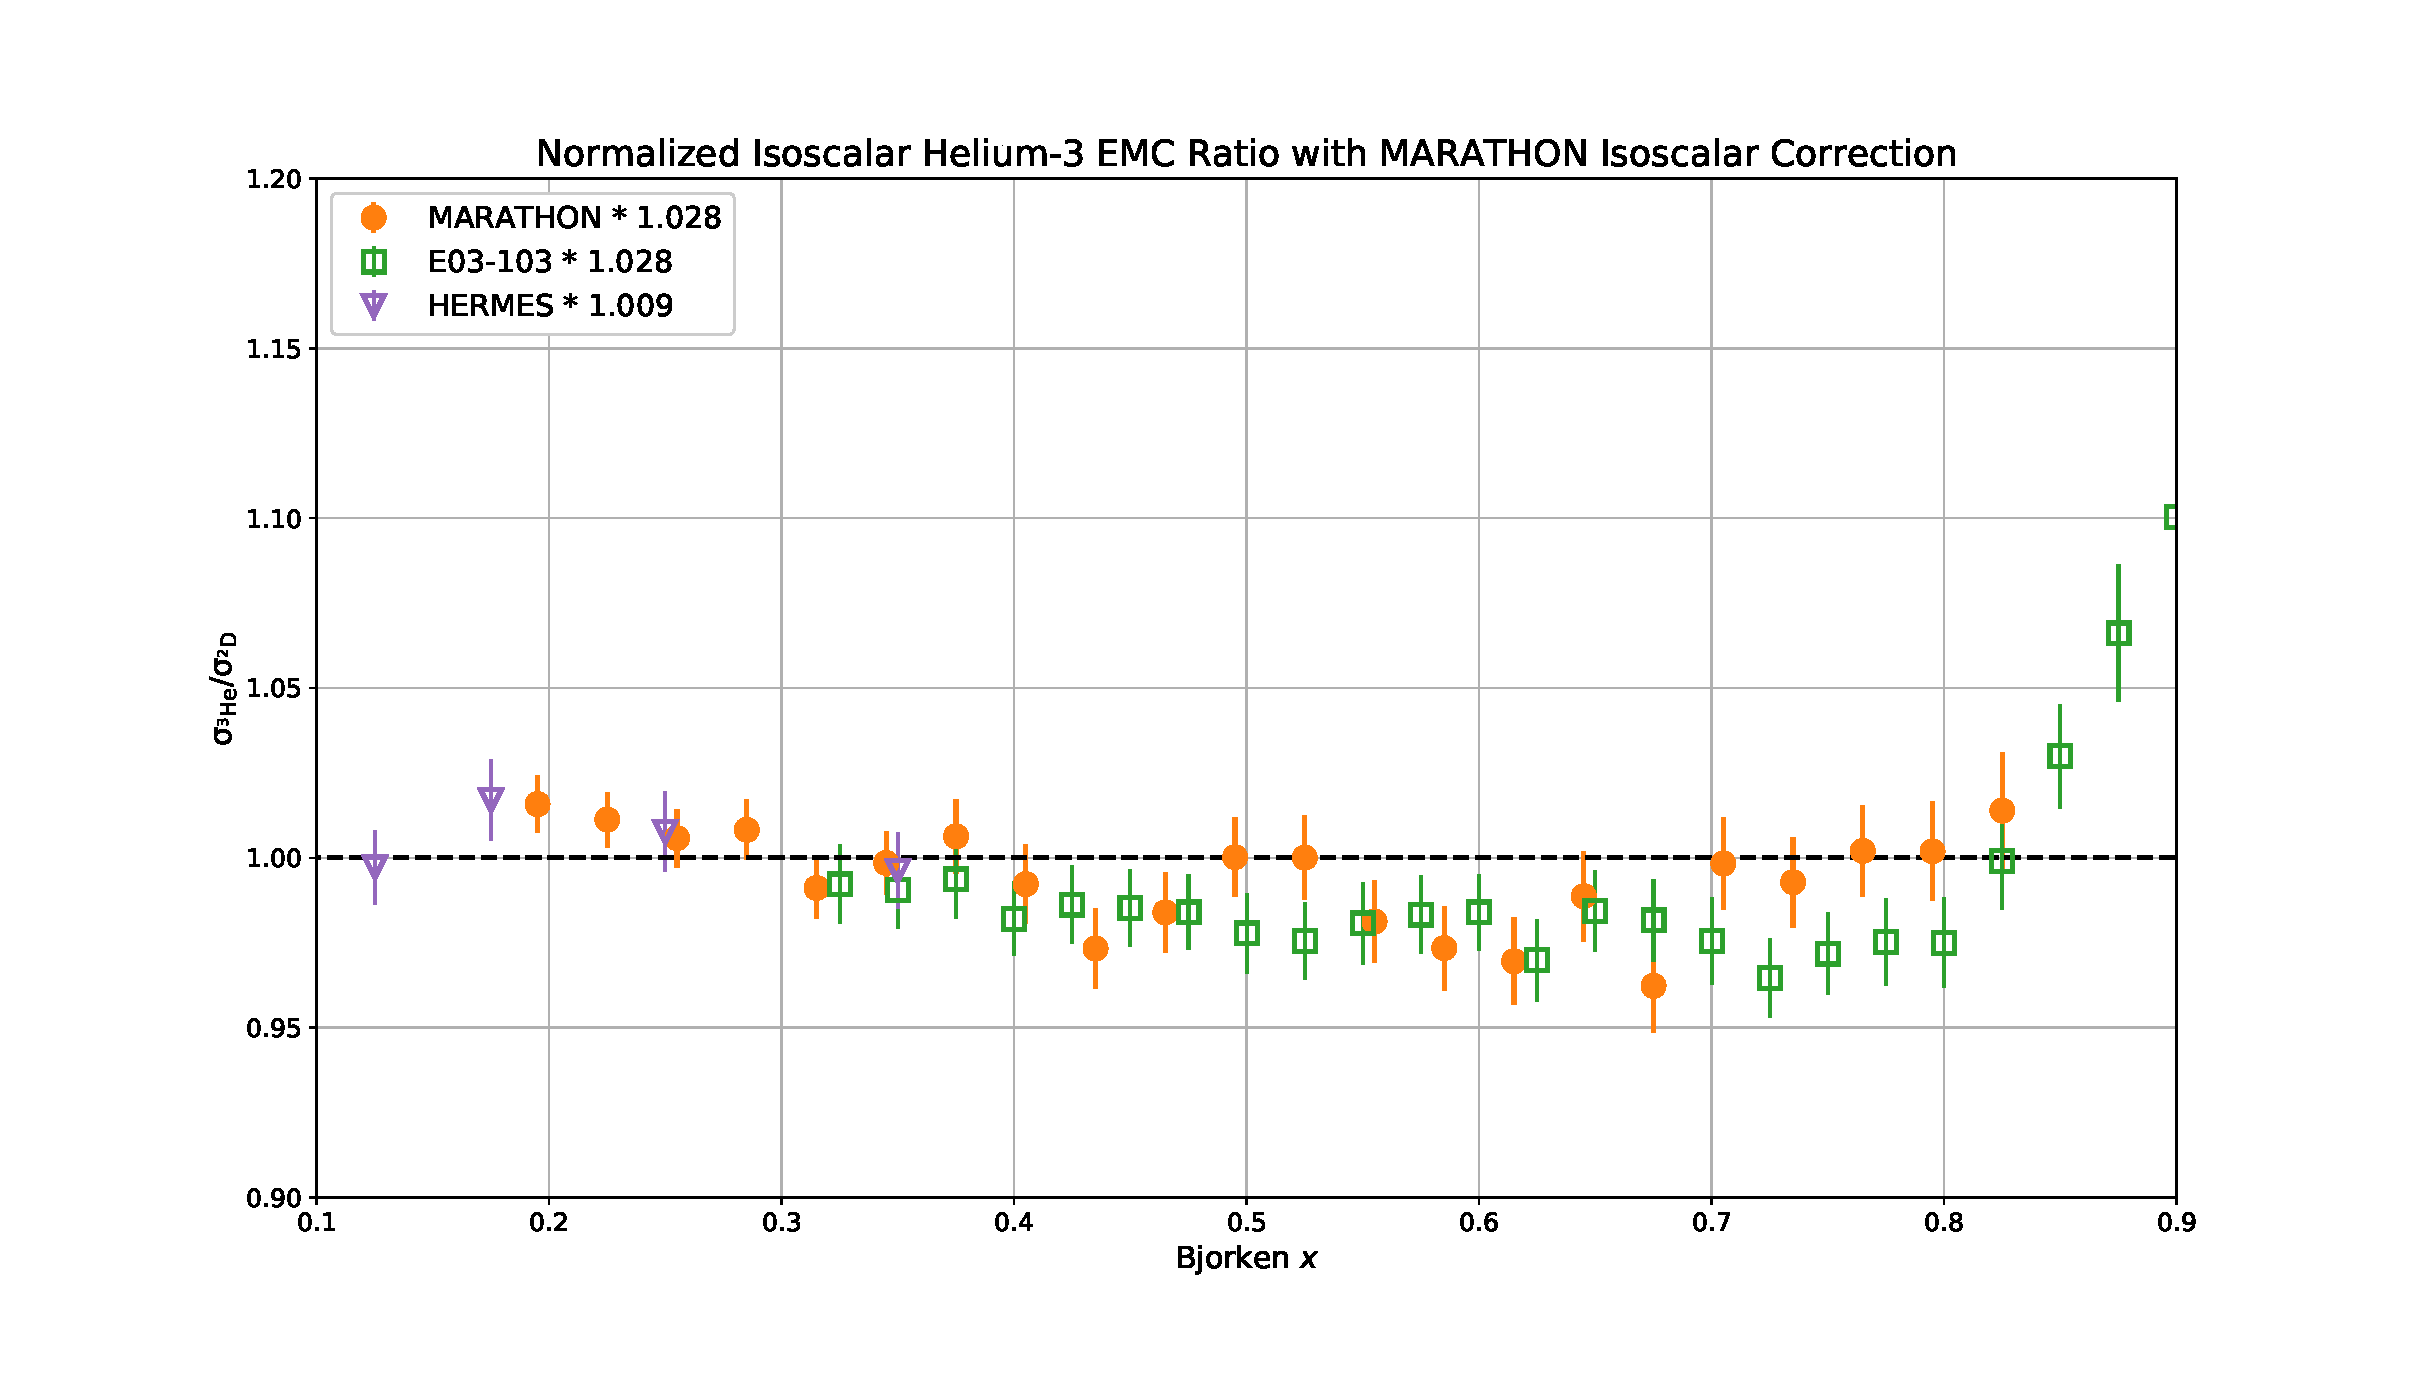
\includegraphics[width=\textwidth]{./results/fig/maraisonorm_comp.eps}
	\caption{A comparison of isoscalar, normalized data from MARATHON, E03-103, and HERMES. The MARATHON isoscalar correction is applied to all data. The MARATHON and E03-103 are normalized by $2.8\%$ and the HERMES data is normalized by $0.9\%$.}
	\label{fig:maraisonormcomp}
\end{figure}

\section{Analyzing the EMC slope}

Studies of the EMC effect often strive to look for correlations between the strength of the EMC effect and other nuclear quantities. To do this, a measure of the EMC strength must be defined. The typical definition of this is the absolute value of the slope of the isoscalar EMC ratio in the range $0.35 \leq x \leq 0.7$, referred to as $\left|dR_{\text{EMC}}/dx\right|$. One benefit of this definition is that it is largely free of normalization uncertainties. 

\begin{figure}[p]
	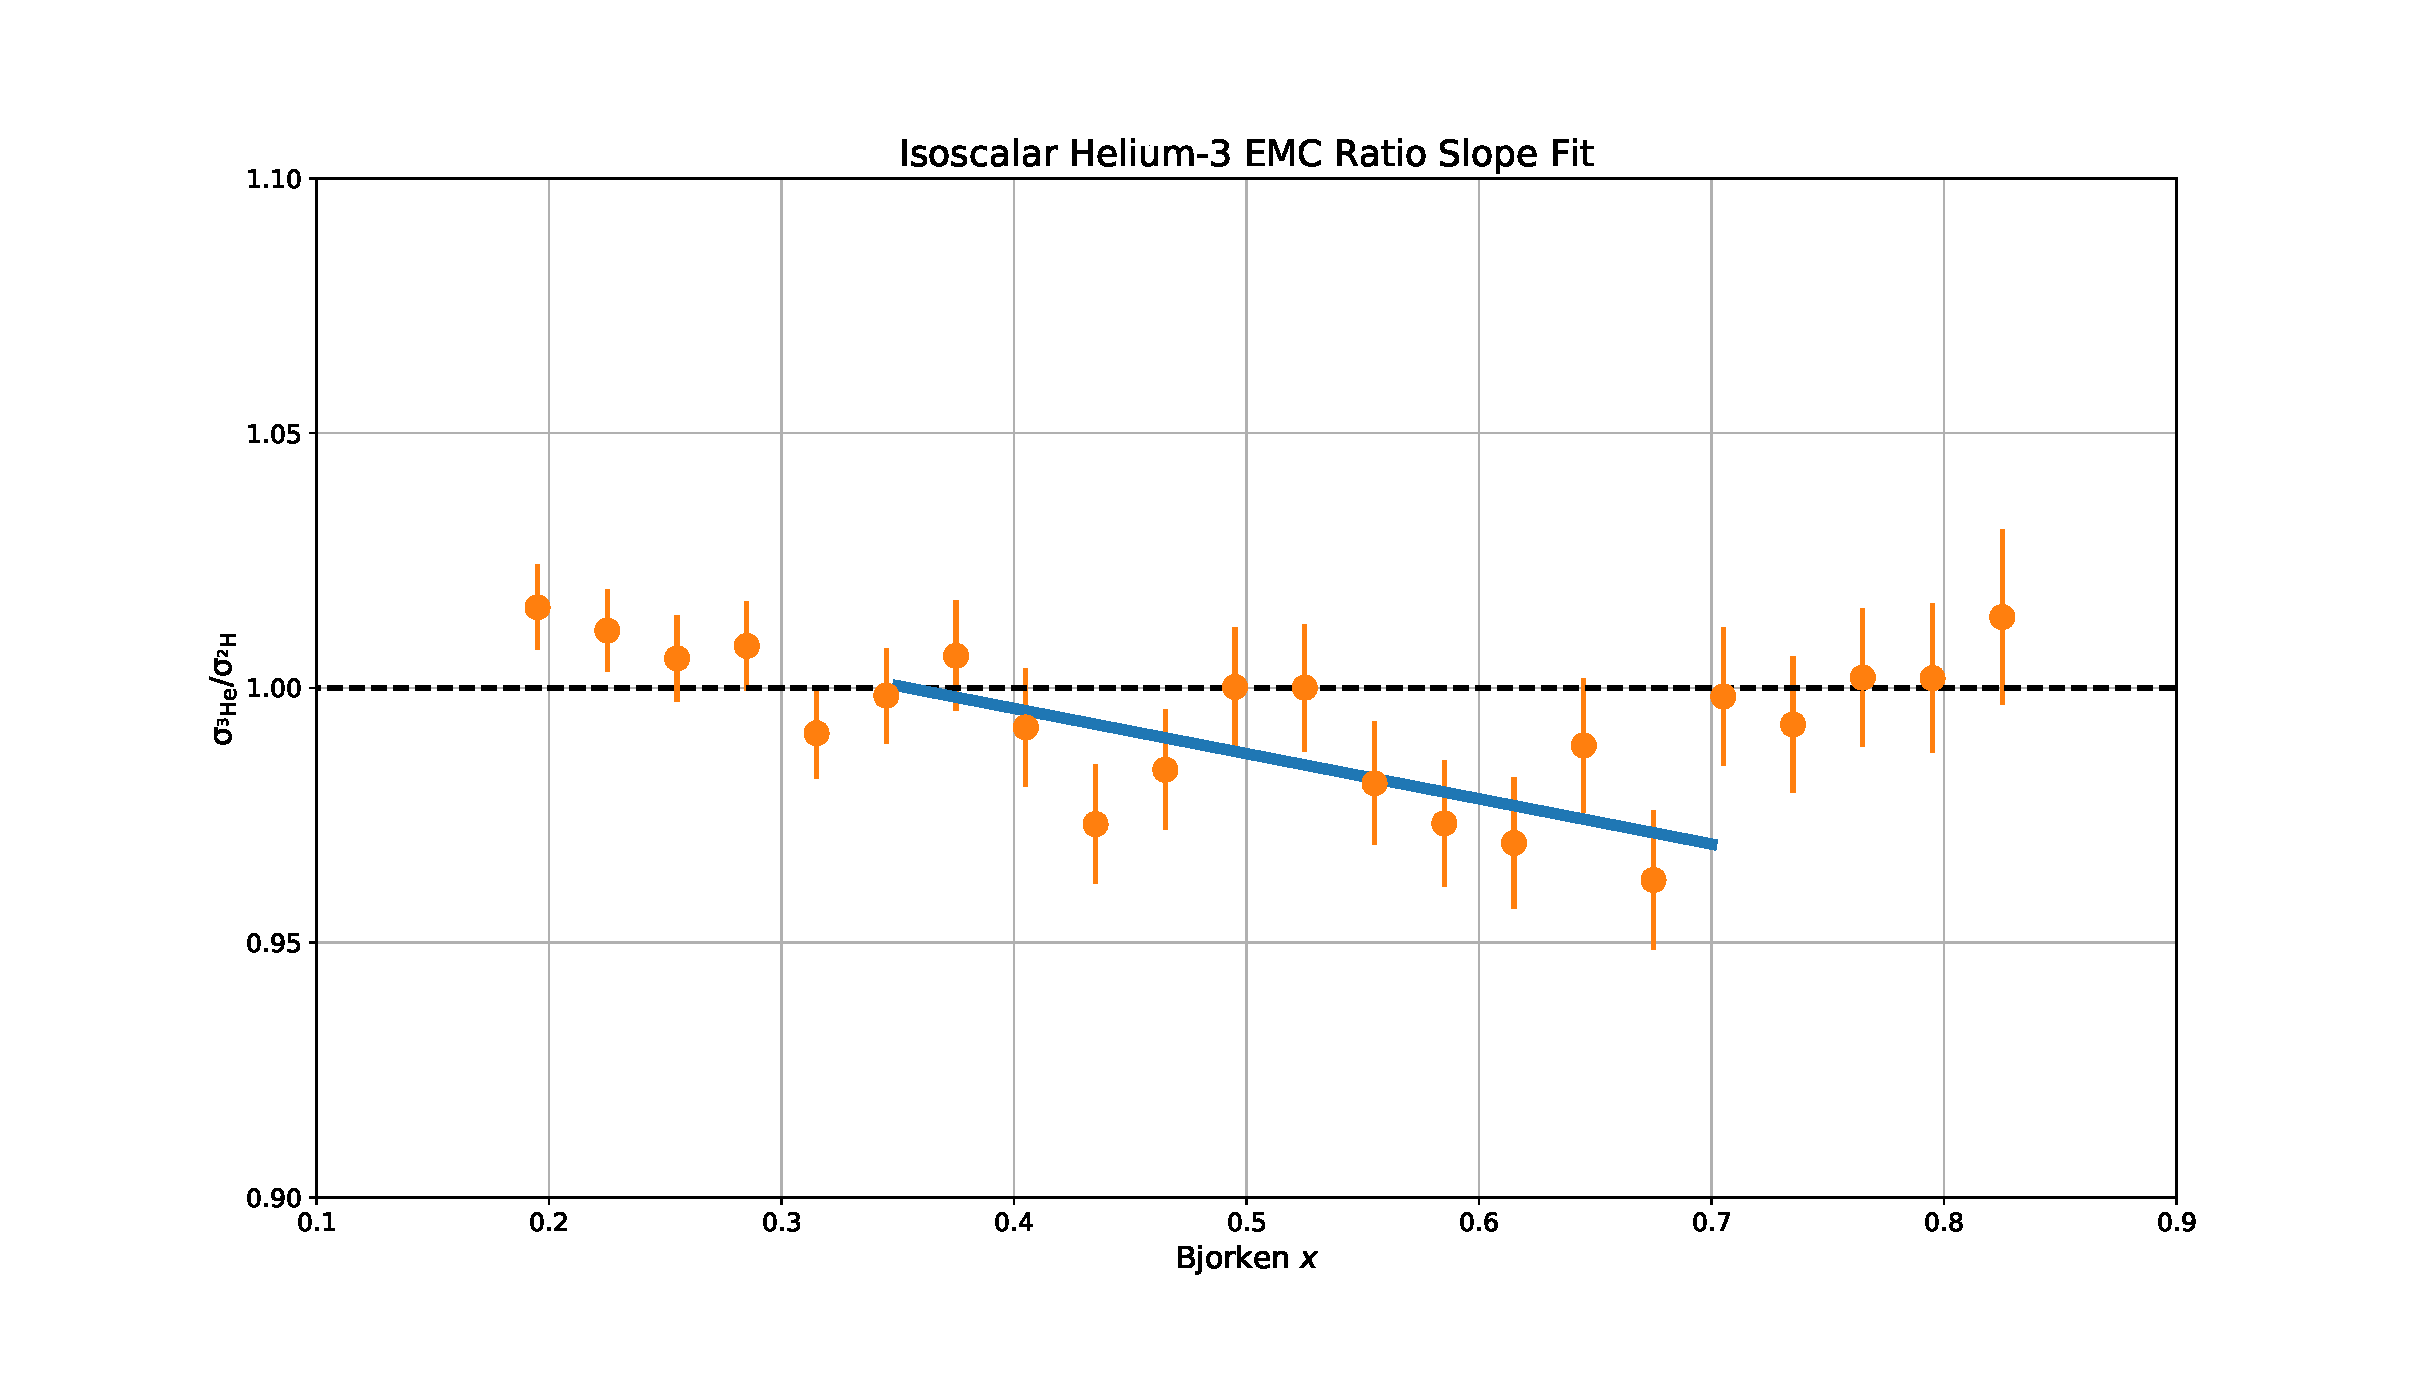
\includegraphics[width=\textwidth]{./results/fig/slope_fit.eps}
	\caption{A fit of the EMC slope of the MARATHON Helium-3 EMC data.}
	\label{fig:slope_fit}
\end{figure}

Figure \ref{fig:slope_fit} shows this fit for the Helium-3 EMC ratio. In selecting the data for the fit, the cut was placed on the range of $0.35 \leq x \leq 0.7$, as defined in the previous paragraph. This has the effect of omitting the bins centered at $x=0.345$ and $x=0.705$. As these bins are close to the fit range and can be considered part of the EMC region, their inclusion was studied. Ultimately, the decision was made to exclude these points in order to maintain consistency with the traditional extraction that only uses data in the defined range. The inclusion of the $x=0.345$ bin resulted in an approximately $5\%$ lowering of the slope. This is a small effect because the bins value is nearly centered within the statistical fluctuations in the data and the EMC slopes are often nearly linear down to approximately $x=0.25$. Inclusion of the $x=0.705$ bin resulted in a nearly $50\%$ decrease in the slope. This is a significantly larger effect. This is because the bin at $x=0.705$ not only appears to have a very large fluctuation from the trend of the data, but this is also the region where Fermi motion begins to flatten out the EMC slope until the data makes a sharp turn upward. The exclusion of these points means that the fit data is in the range of $0.36 \leq x \leq 0.69$.

In this section the data is shown along with other EMC data to study correlations with nuclear quantities. These data are from the SLAC E139, JLab E03-103, and CLAS experiments. Extractions of the EMC slopes from these data have been completed by both Arrington \textit{et. al.} \cite{arrington_src} and Malace \textit{et. al.} \cite{malace_emc}. Each of these experiments and extractions use a different isoscalar correction, which has an effect on the extracted slope. In order to ensure that correlations are properly examined, isoscalar corrections should be applied in a consistent way to all data. For the following plots (Figures \ref{fig:emc_v_A}-\ref{fig:emc_v_a2}), the data from each of these experiments has the MARATHON $F_2^n/F_2^p$ based isoscalar correction applied. The EMC slopes are then extracted by a linear fit of the data in the $0.35 \leq x \leq 0.7$ region. Due to binning, the range of data included for E139 is $0.36 \leq x \leq 0.68$. Due to binning and available data, the range of data included for CLAS is $0.353 \leq x \leq 0.58$.

The two most commonly studied correlations are with mass number $A$ and scaled nuclear density. Nuclear density, measured in nucleons/fm$^{3}$, is the number of nucleons per unit volume of the nucleus. In this analysis, the nuclear density is calculated using the hard sphere approximation, $\rho\left(A\right) = 3A/4\pi R^3$. In this equation, $R^2=5\left<r^2\right>/3$, where $\left<r^2\right>$ is the rms charge radius of the nucleus being studied. The rms charge radii used come from \cite{DeVries} which are extracted from electron scattering experiments. In cases where multiple values are listed, the average of the values are used. The exception to this is Silver-108 (Ag108), as charge radius data for this nucleus is unavailable. Nuclear charge radius is correlated with $A$, so to approximate the charge radius of Ag108, the charge radii of Ag107 and Ag109 from \cite{2012_charge_radii} were averaged. Scaled nuclear density is the nuclear density scaled by a factor of $\left(\text{A}-1\right)$/A. This scaling removes the struck nucleons contribution to the density from the value. The correlation of the EMC effect with nuclear density has been noticed in many past experiments, as described in Chapter \ref{chap:emc}. Figures \ref{fig:emc_v_A} and \ref{fig:emc_v_snd} show the correlation with $A$ and scaled nuclear density, respectively.

\begin{figure}[p]
	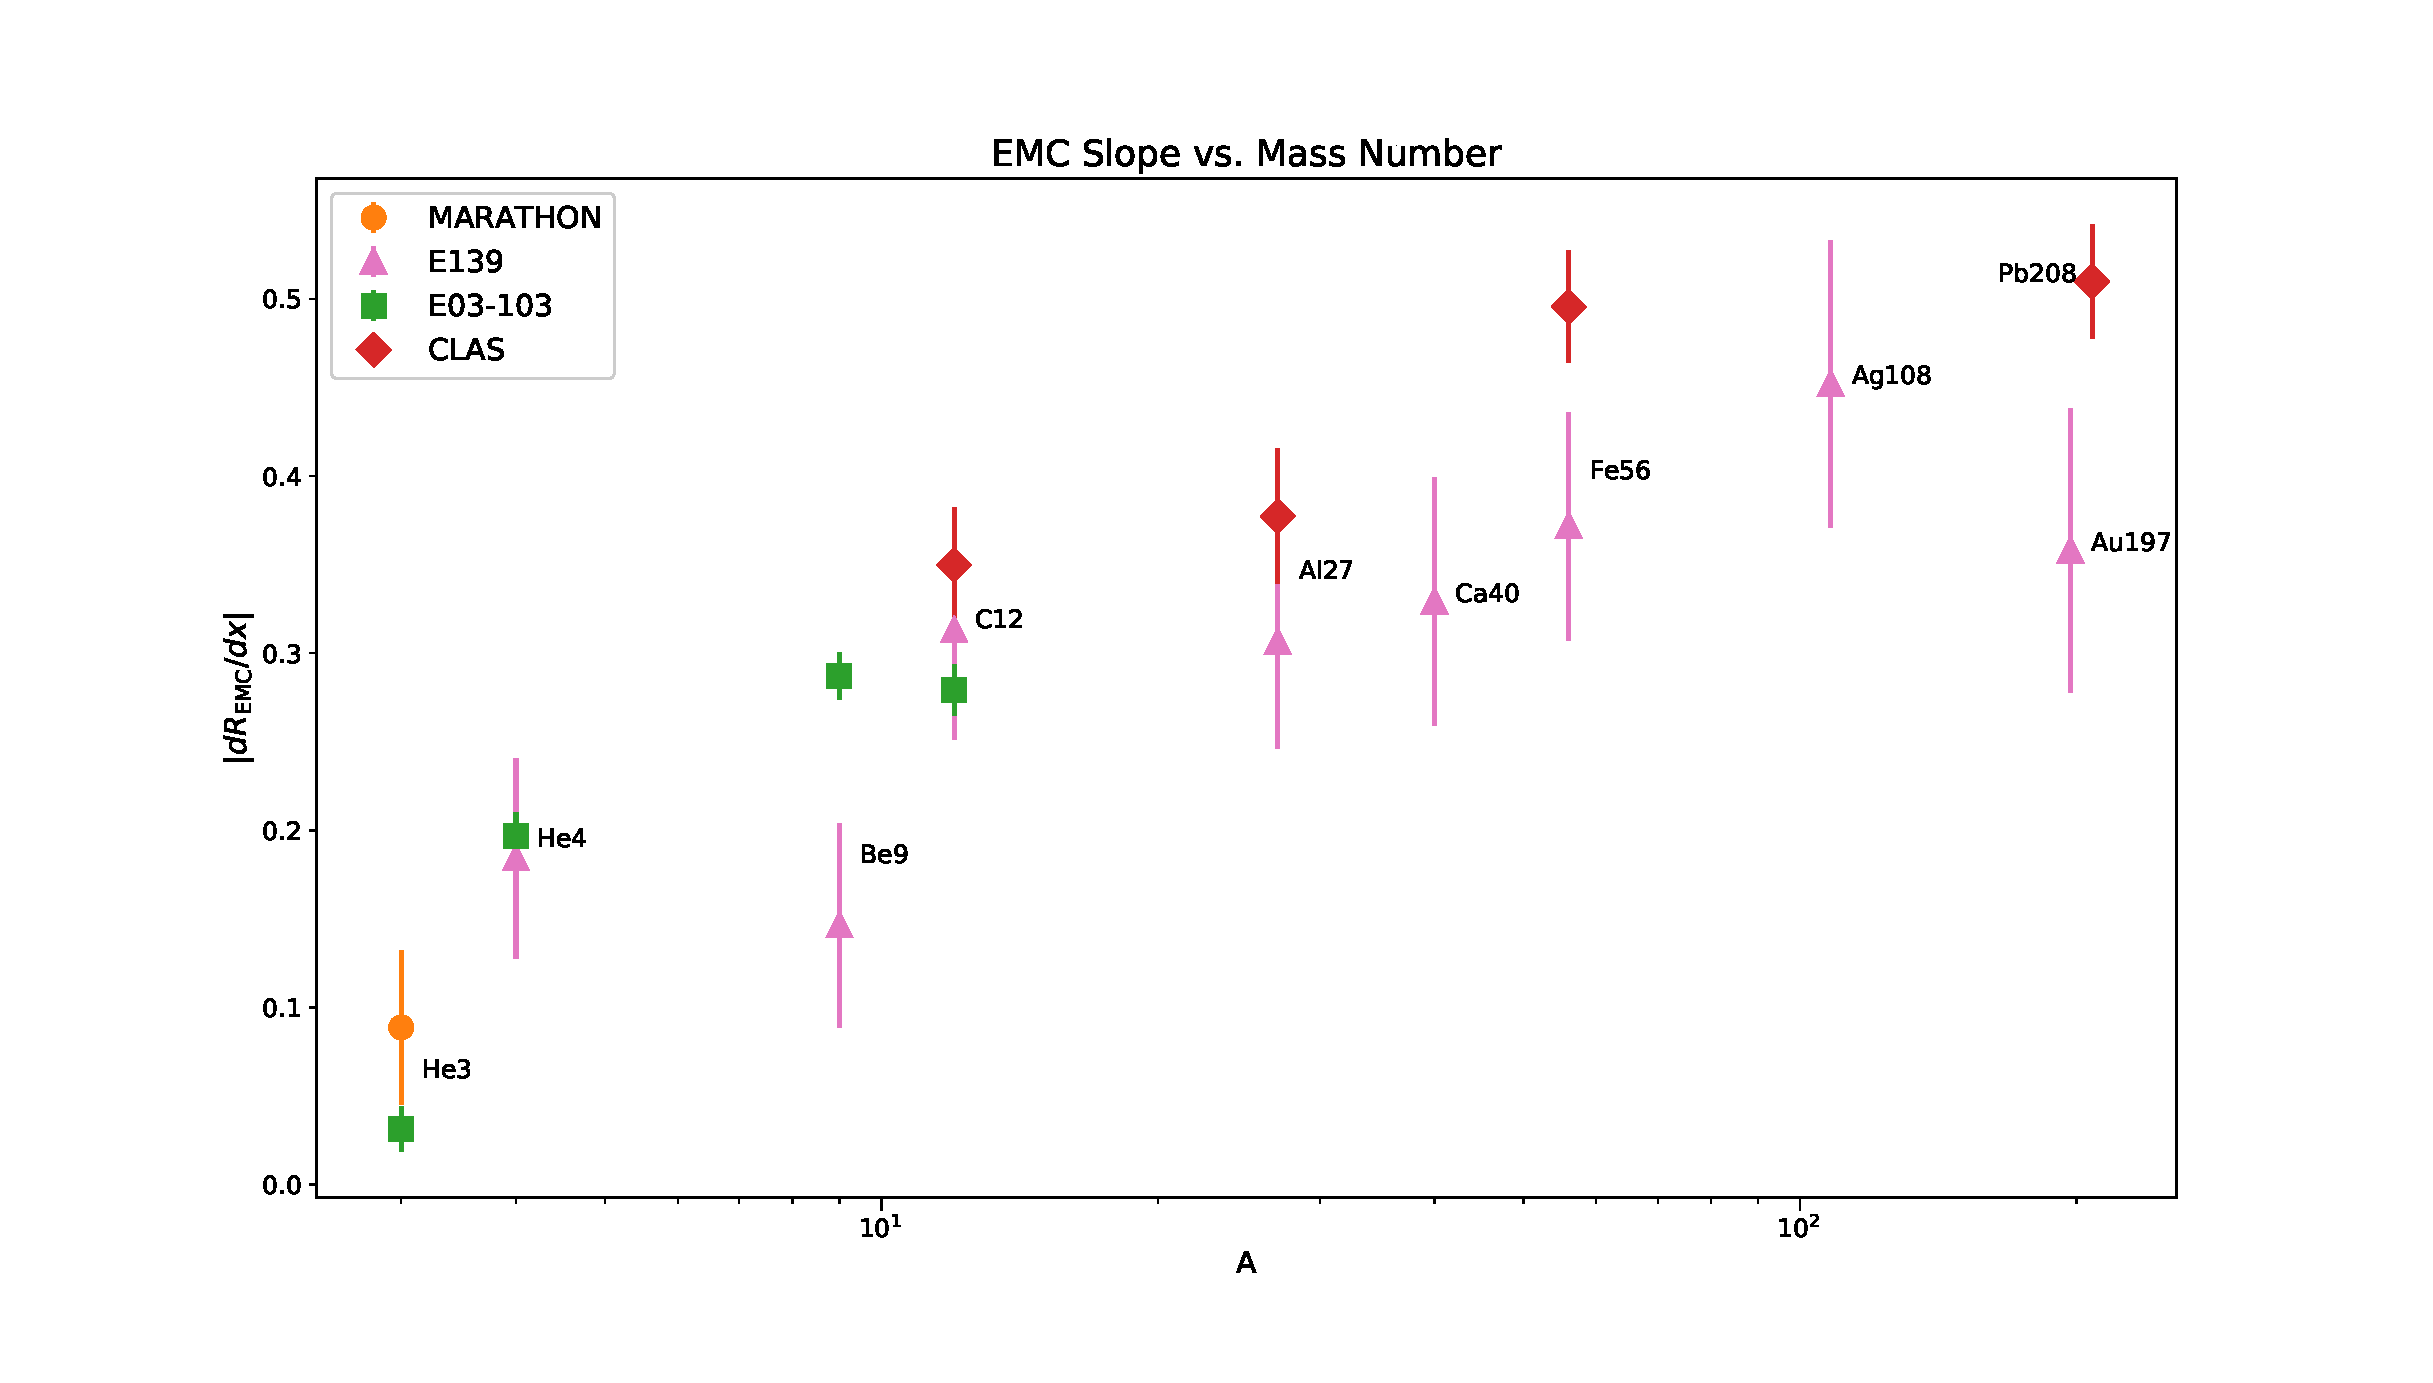
\includegraphics[width=\textwidth]{./results/fig/EMC_vs_A.eps}
	\caption{This plot shows EMC slope versus mass number $A$ for a selection of nuclei.}
	\label{fig:emc_v_A}
\end{figure}

\begin{figure}[p]
	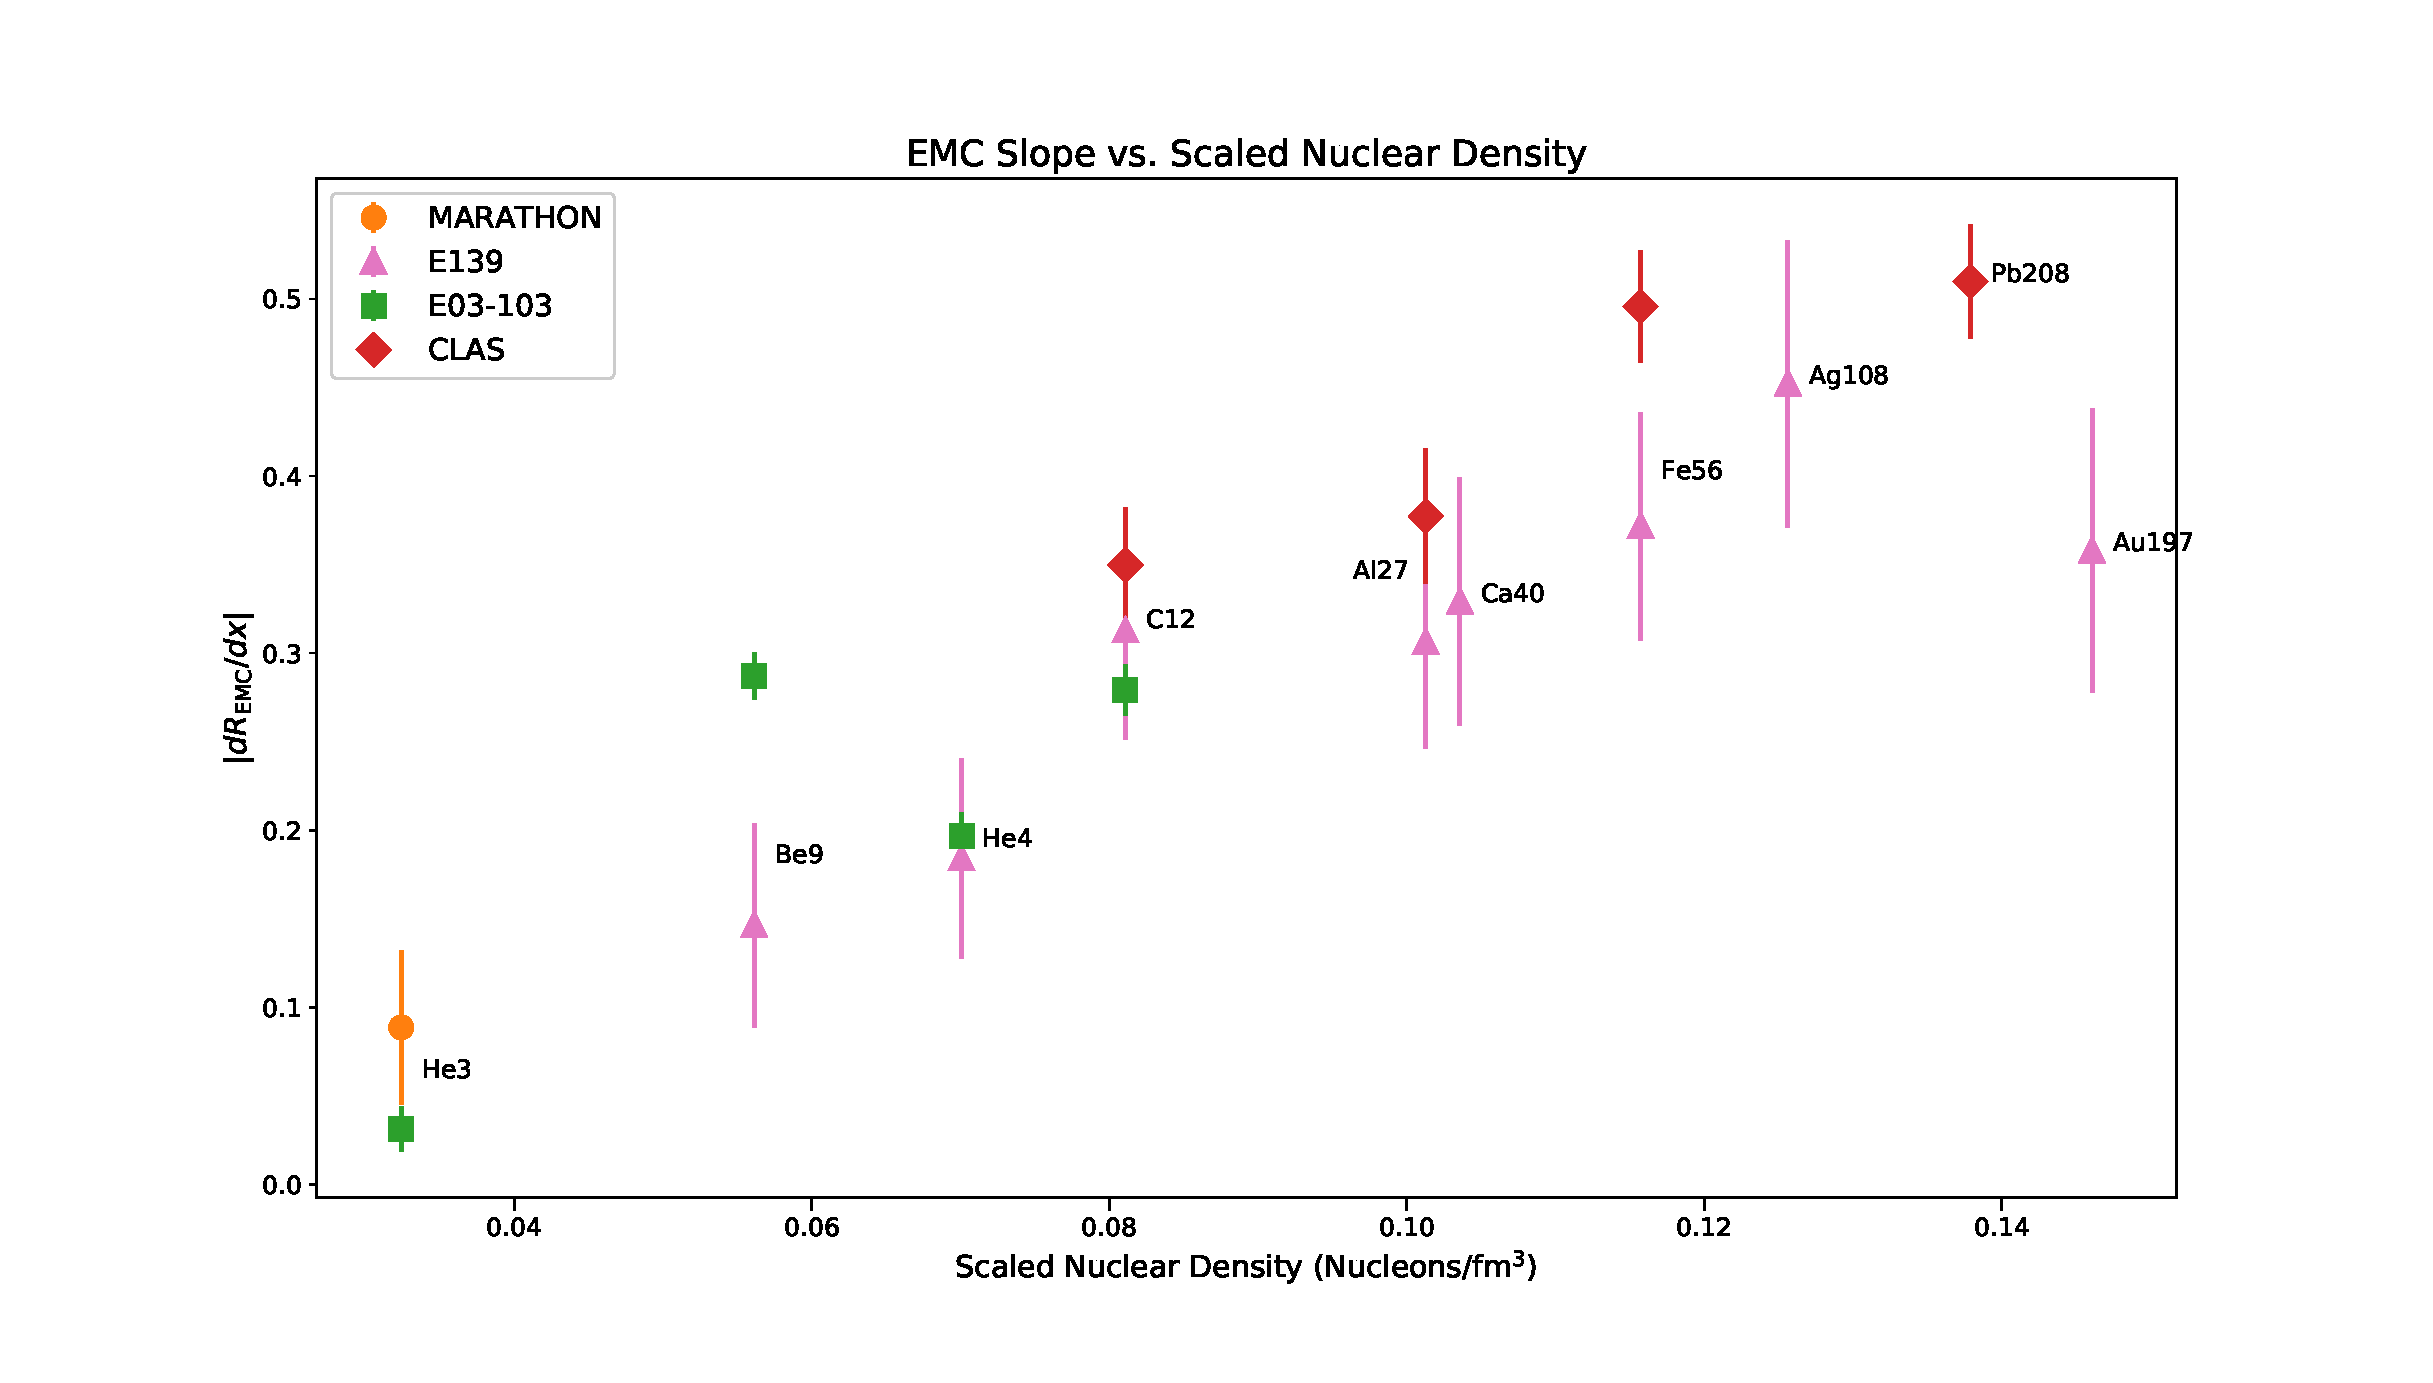
\includegraphics[width=\textwidth]{./results/fig/EMC_vs_SND.eps}
	\caption{This plot shows EMC slope versus scaled nuclear density for a selection of nuclei.}
	\label{fig:emc_v_snd}
\end{figure}

Reference \cite{slope_predict} examines the correlation of the EMC slope with nuclear binding energy per nucleon and the residual strong interaction energy (RSIE) per nucleon. Nuclear binding is typically understood to play a part in the EMC effect, but is considered insufficient to completely explain the effect. The RSIE is defined as the energy loss of nucleons binding together by strong interaction. RSIE is calculated by removing the Coulomb contribution to the binding energy of the nucleus. That is, $RSIE\left(A,Z\right) = B\left(A,Z\right) + \left(0.71 \text{MeV}\right)Z\left(Z-1\right)A^{-\nicefrac{1}{3}}$ where $B\left(A,Z\right)$ is the binding energy of the nucleus. This calculation assumes that nuclear binding is only comprised of strong and electro-magnetic interactions. For these figures and calculations, the binding energies from \cite{BindingEnergy} are used. Figures \ref{fig:emc_v_be} and \ref{fig:emc_v_rsie} show the correlation with binding energy per nucleon and RSIE per nucleon, respectively.

\begin{figure}[p]
	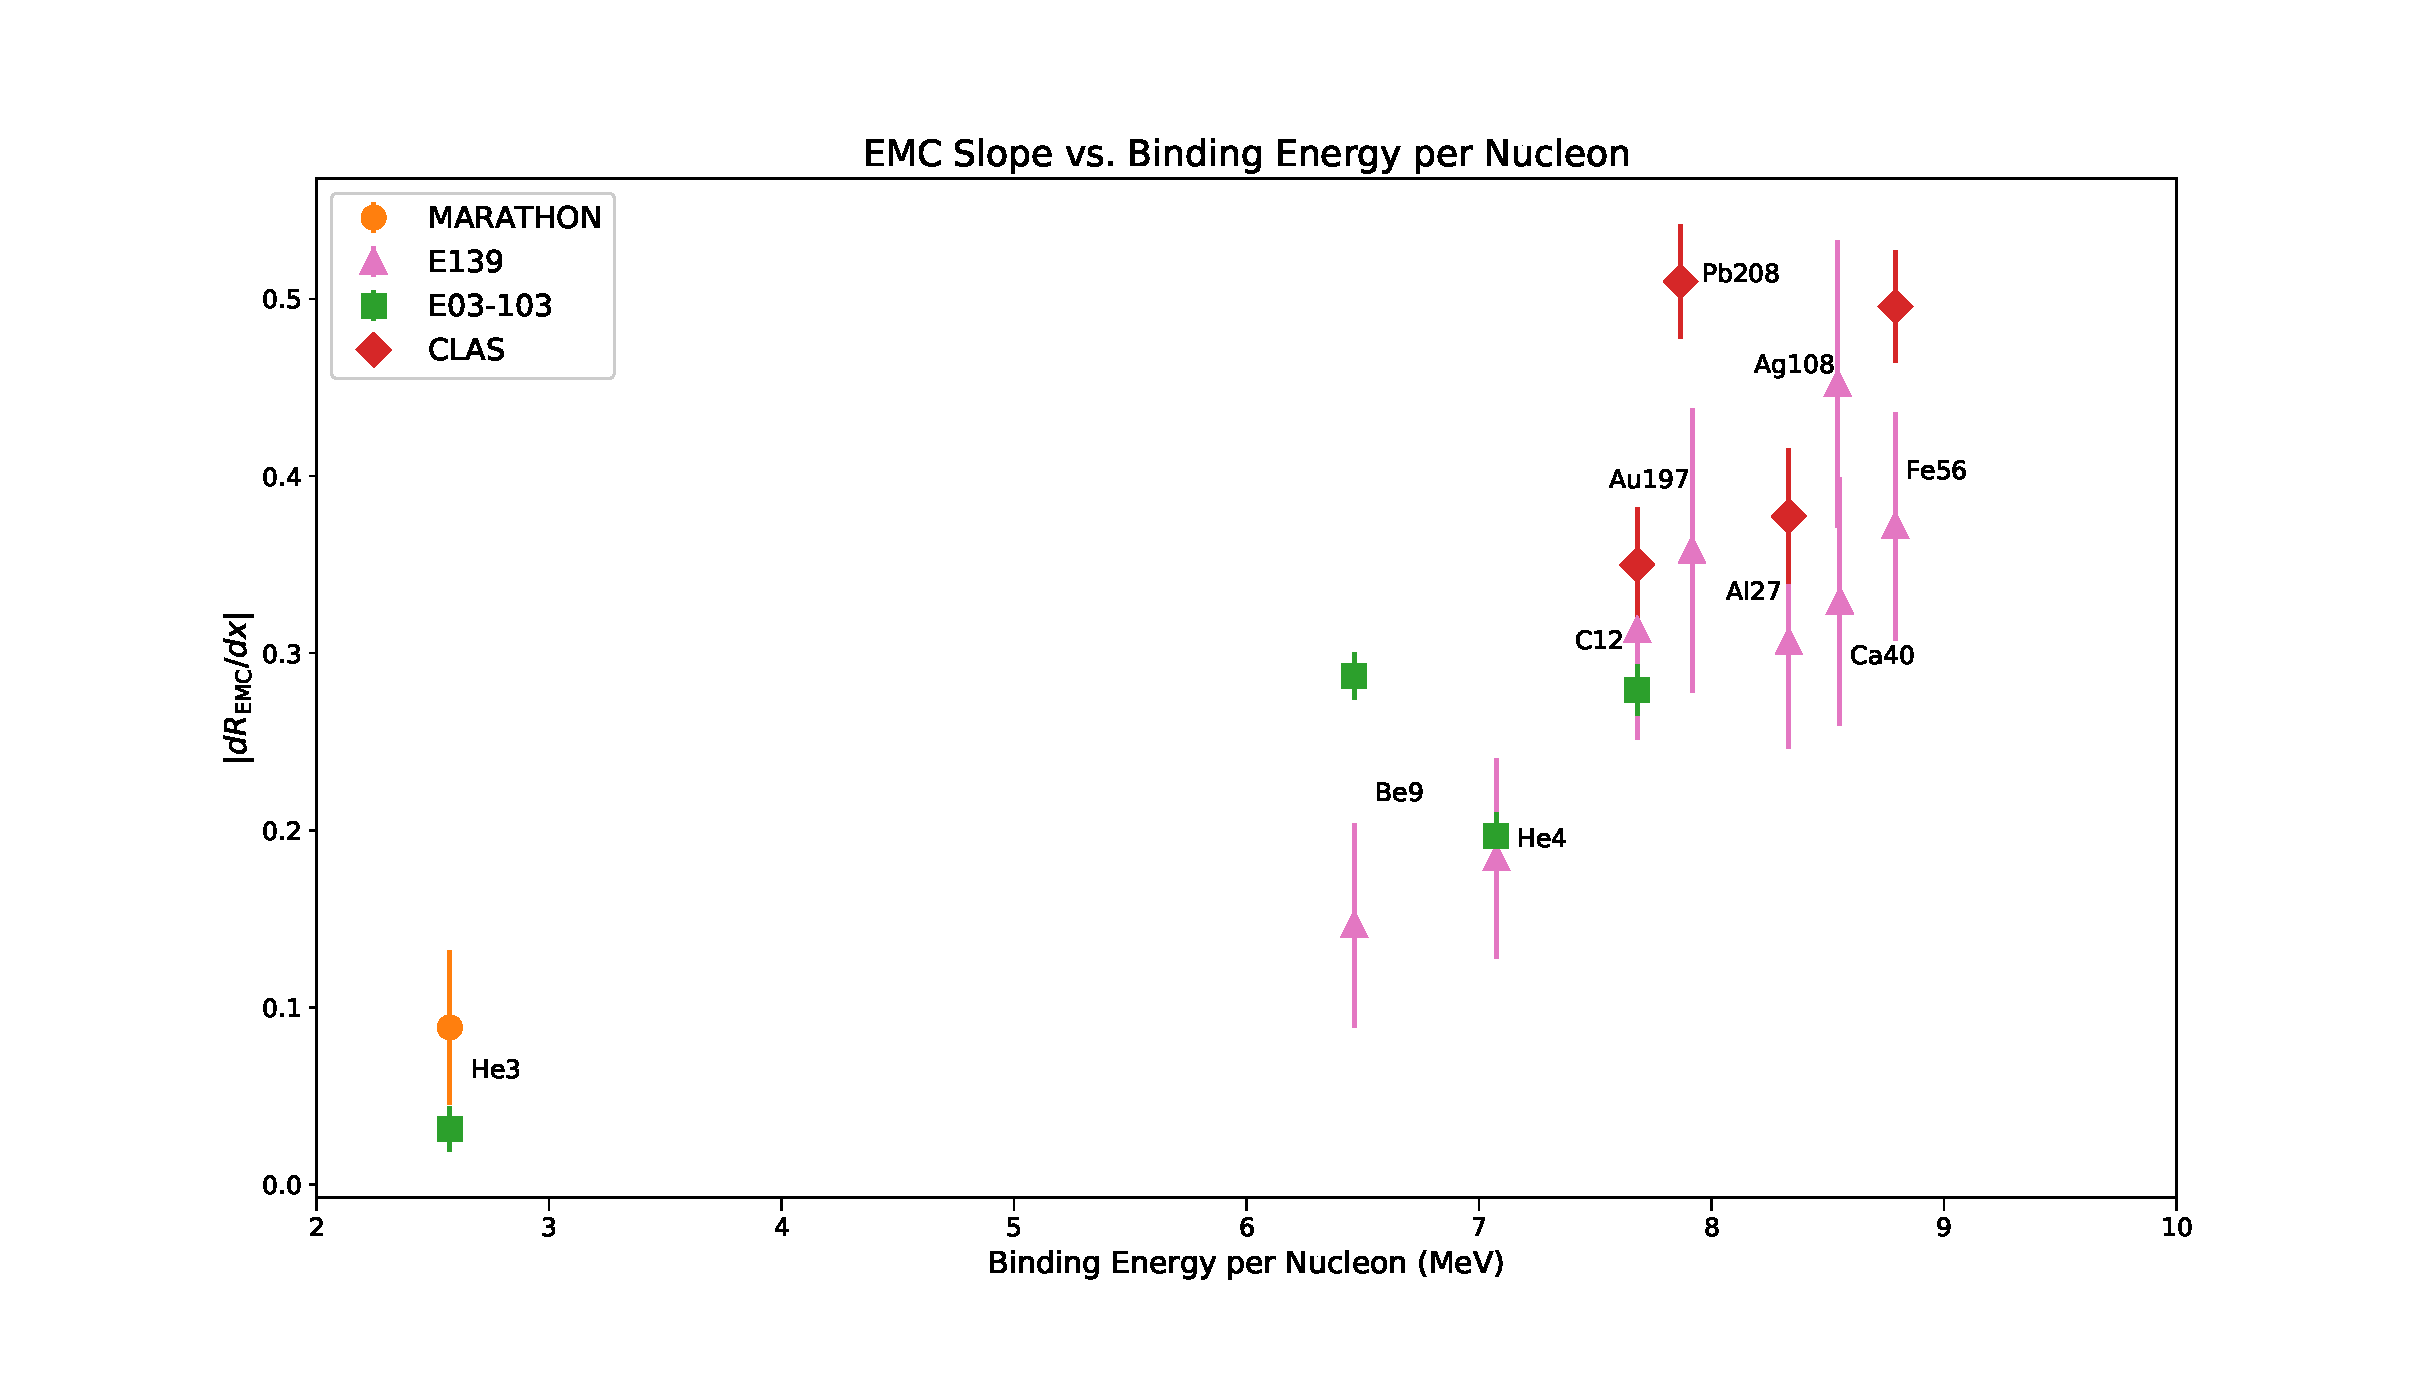
\includegraphics[width=\textwidth]{./results/fig/EMC_vs_BE.eps}
	\caption{This plot shows EMC slope versus binding energy per nucleon for a selection of nuclei.}
	\label{fig:emc_v_be}
\end{figure}

\begin{figure}[p]
	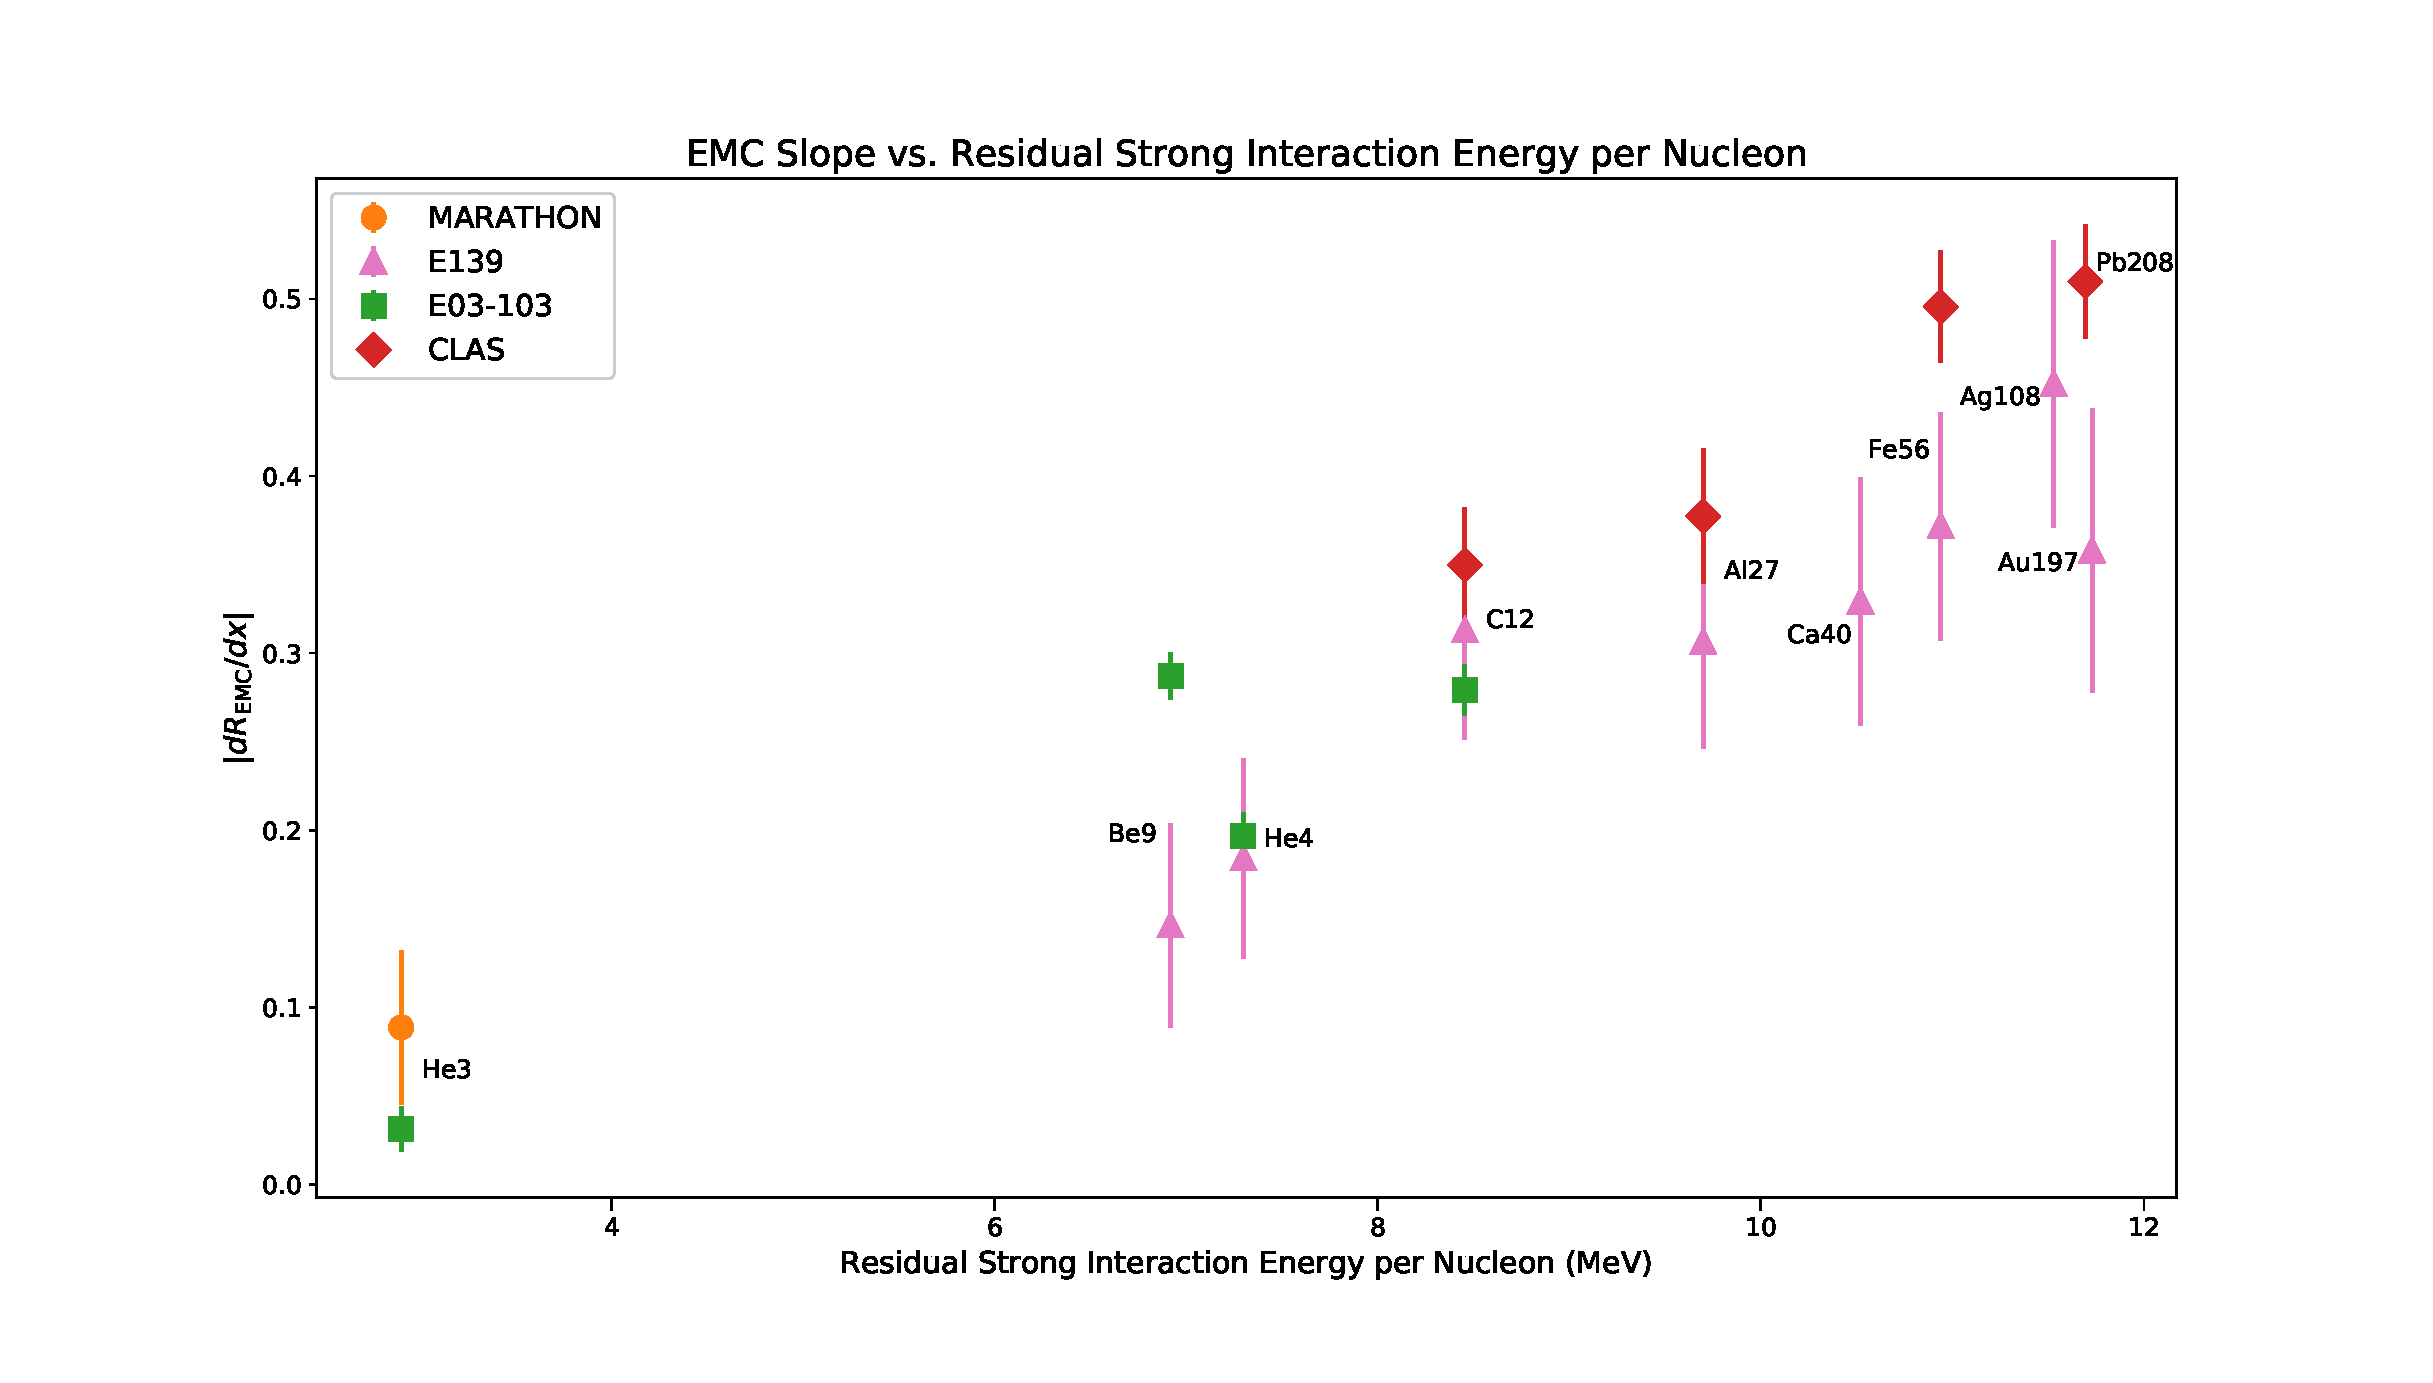
\includegraphics[width=\textwidth]{./results/fig/EMC_vs_RSIE.eps}
	\caption{This plot shows EMC slope versus residual strong interaction per nucleon energy for a selection of nuclei.}
	\label{fig:emc_v_rsie}
\end{figure}

Another correlation often studied is with the average nucleon separation energy, $\left<\epsilon\right>$. This value is another means of examining the nuclear binding model in the context of the EMC effect. In this scheme, nuclear binding causes the nucleons to have a level of ``off-shellness''. The separation energy of a nucleon is a measure of how off-shell the nucleon is. The separation energy needed causes a rescaling of $x$ by approximately $\left<\epsilon\right>/m$, where $m$ is the mass of the nucleon. Nucleon separation energy is at the heart of models that include off-shell corrections. Off-shell corrections have been shown to well-approximate the shape of the EMC effect, though they cannot describe the effect on their own. The $\left<\epsilon\right>$ values used here were obtained from \cite{arrington_src}. Figure \ref{fig:emc_v_nsep} shows this correlation. Nuclear separation energy data for Lead-208 is unavailable and is thus excluded from this figure.

\begin{figure}[p]
	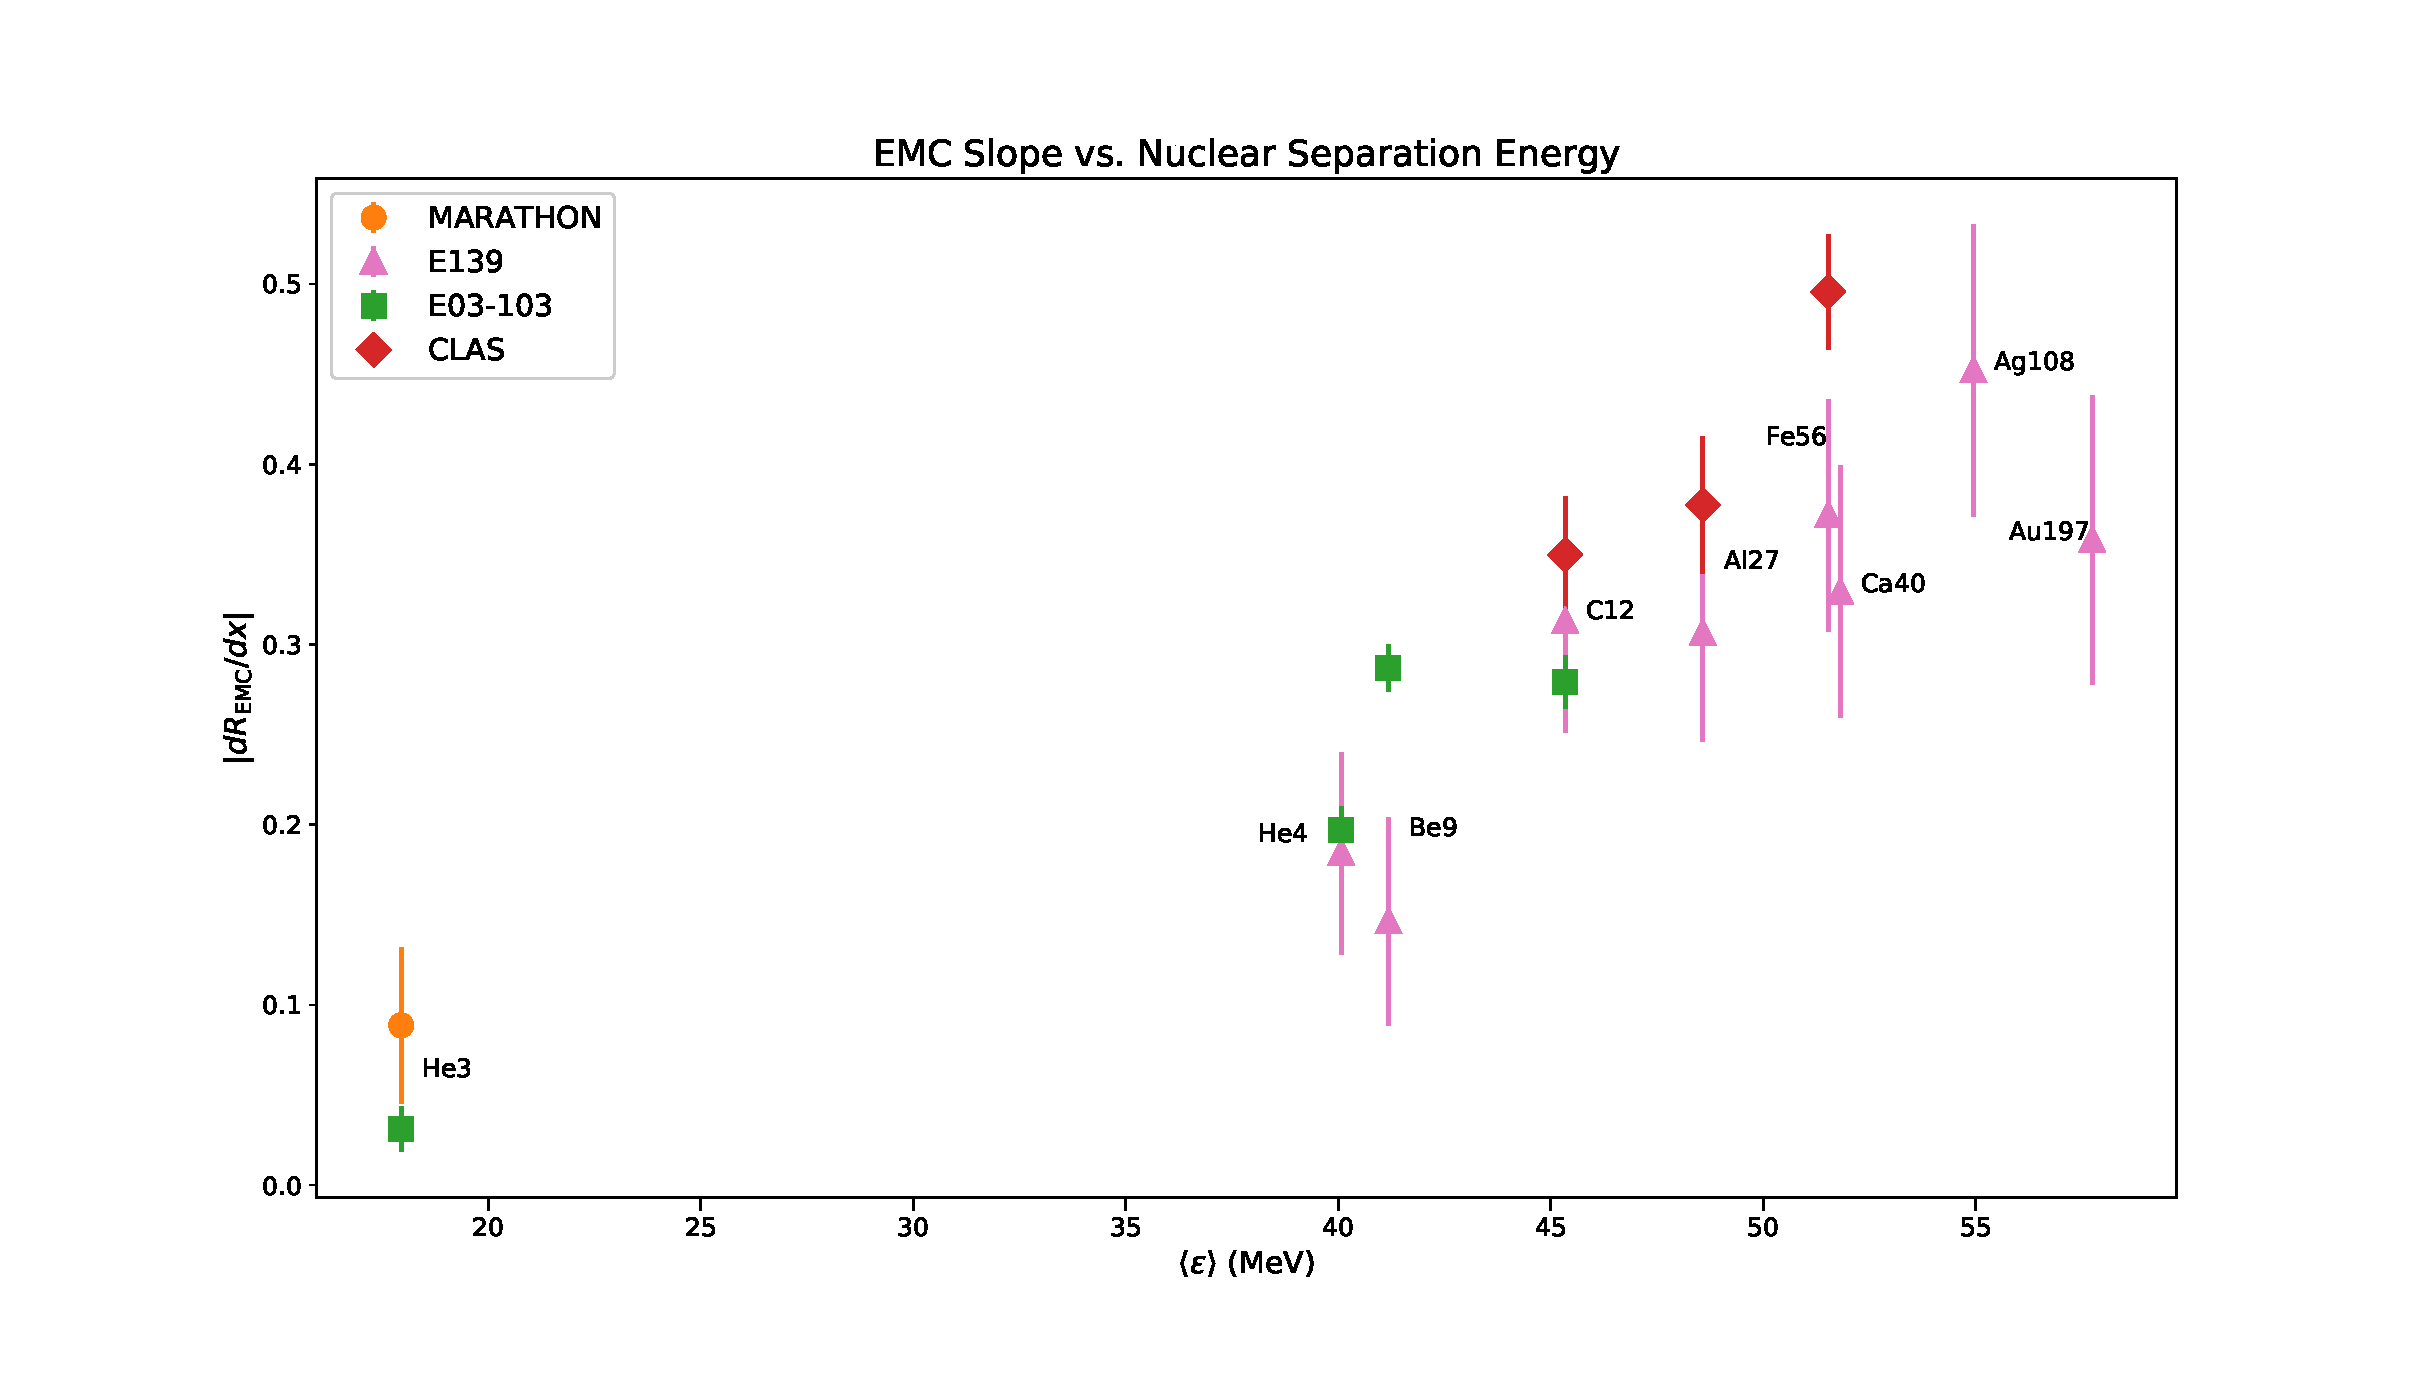
\includegraphics[width=\textwidth]{./results/fig/EMC_vs_NSep.eps}
	\caption{This plot shows EMC slope versus nuclear separation energy for a selection of nuclei.}
	\label{fig:emc_v_nsep}
\end{figure}

The final correlation looked at is with the Short-Range Correlation Scaling Coefficient, $a_2$. In the SRC model, correlated pairs of nucleons are greatly modified giving rise to the EMC effect. A measure of the probability that a nucleon belongs to a nucleon-nucleon SRC pair can be obtained by measuring $a_2$. $a_2$ is the height of a plateau observed when studying the per-nucleon cross section ratio of a nuclear target to that of deuterium in the $Q^2 > 1.4 \text{GeV}^2$ and $1.5 \leq x \leq 1.9$ range. The $a_2$ values used were obtained from \cite{arrington_src}, as it has the most complete set. This ensures that the extractions were treated accordingly. $a_2$ data for Lead-208 only available in \cite{clas_emc}, so that measurement is used here. Figure \ref{fig:emc_v_a2} shows this correlation. There have been no measurements of $a_2$ for Calcium-40 and Silver-108, so they are excluded from the plot.

\begin{figure}[p]
	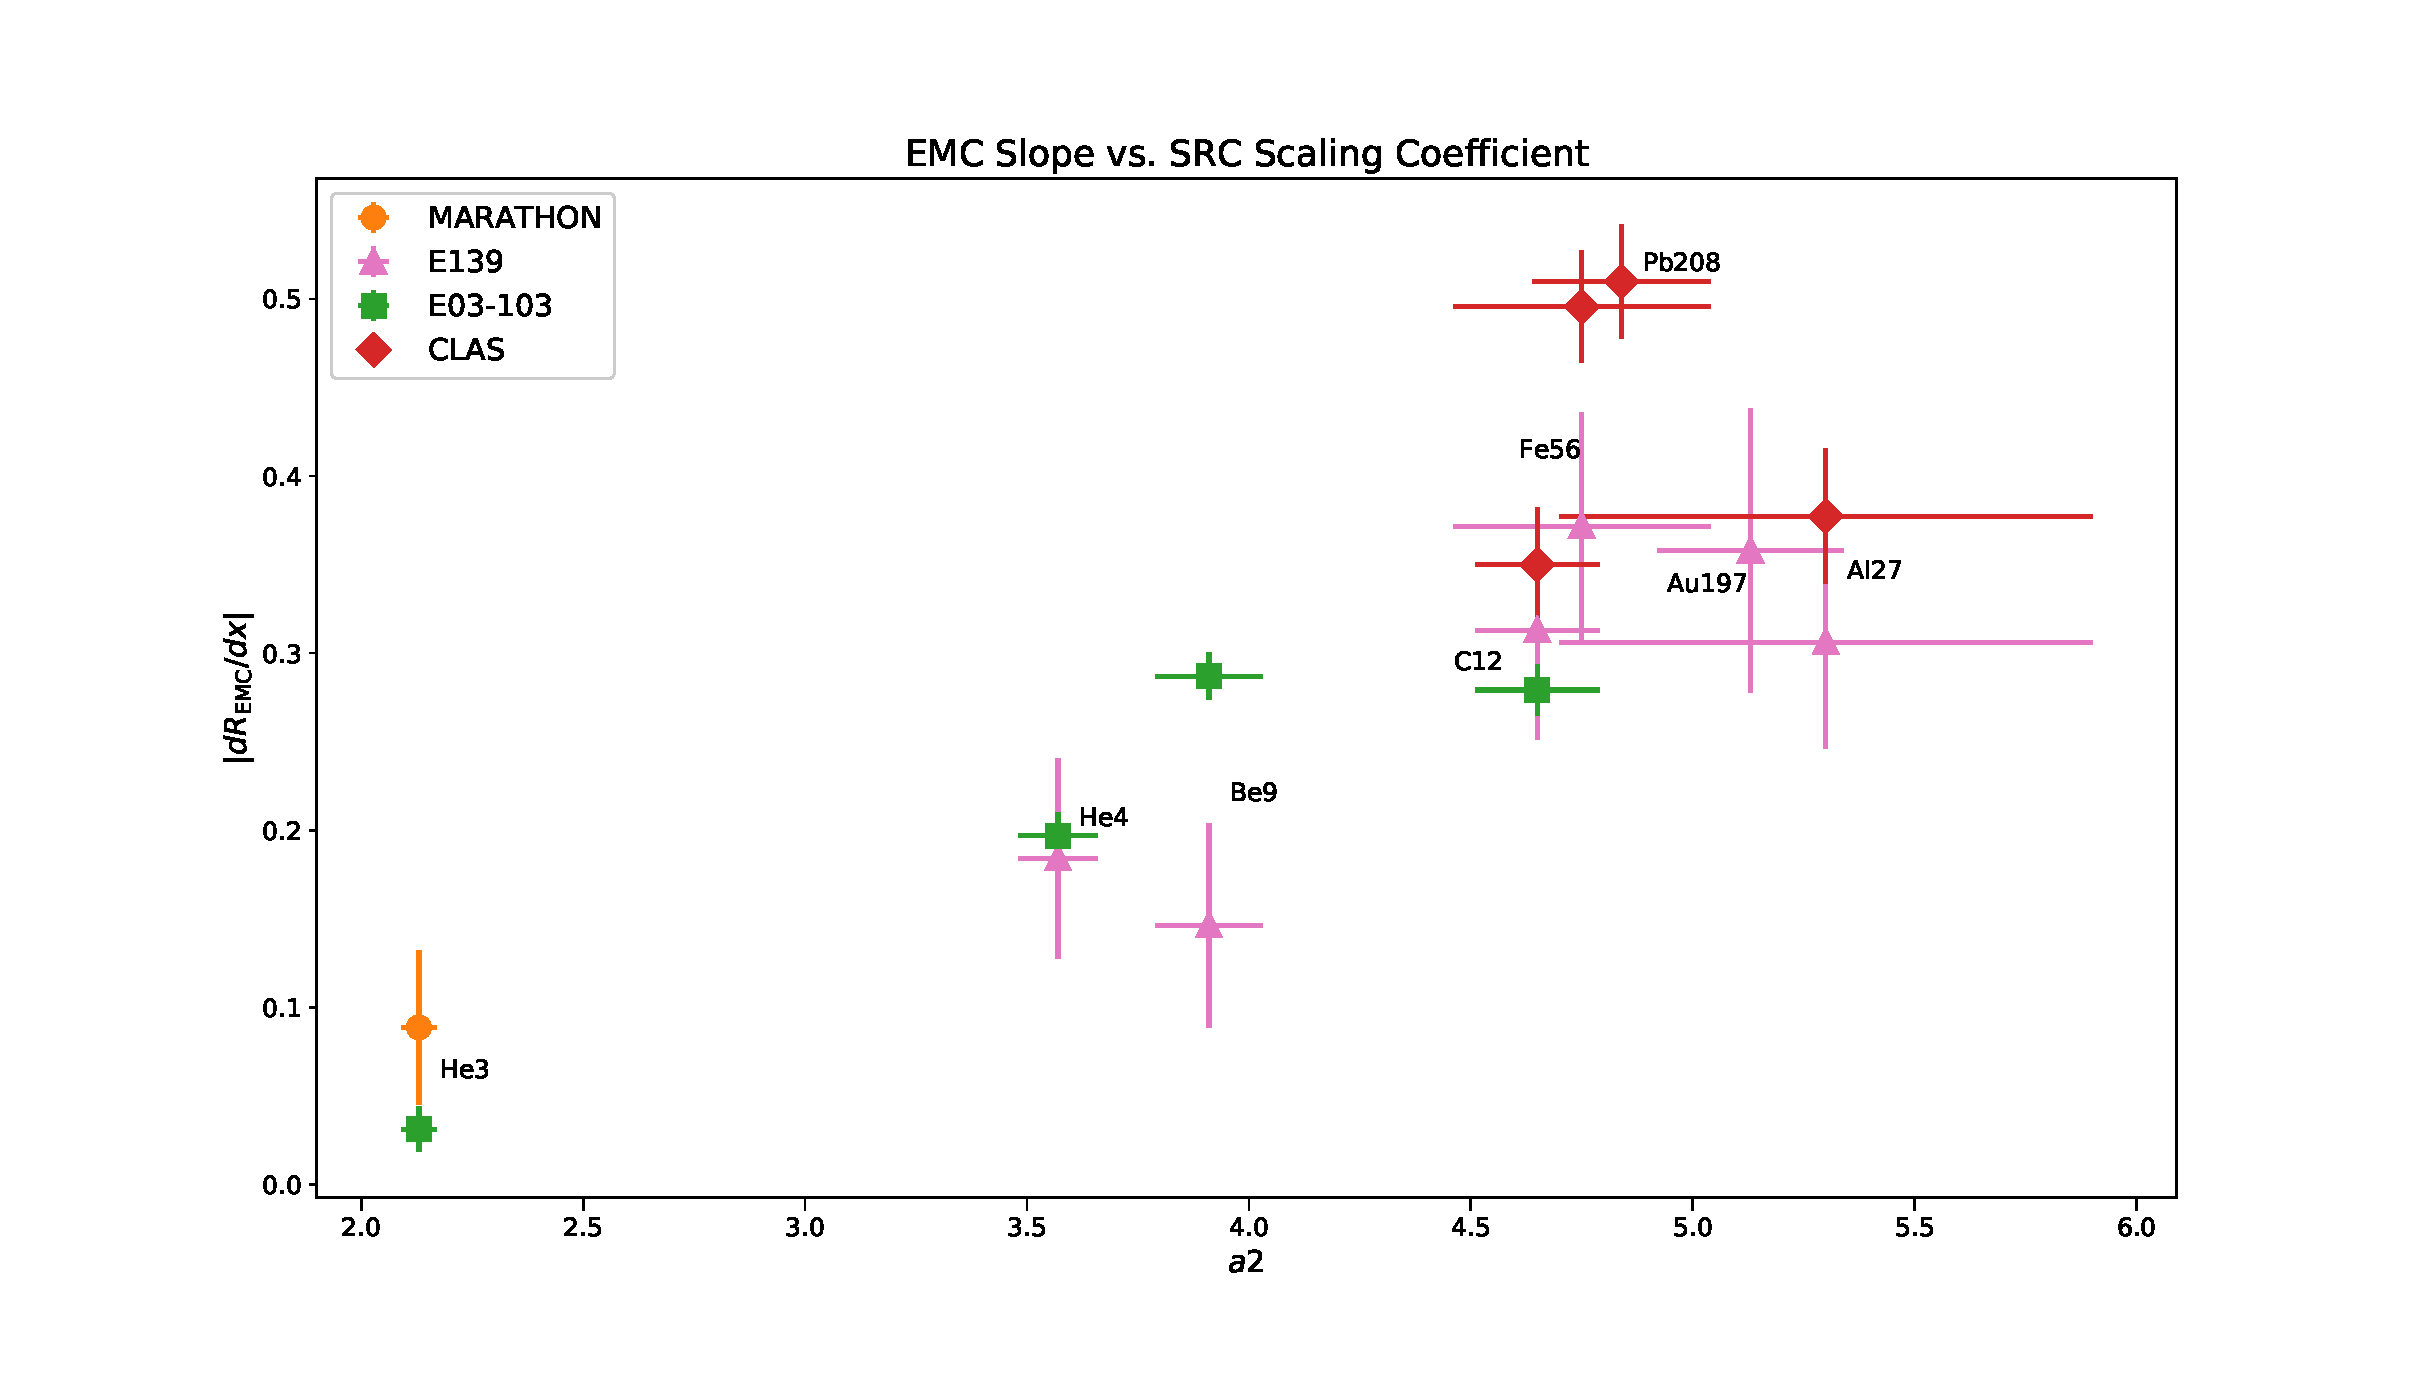
\includegraphics[width=\textwidth]{./results/fig/EMC_vs_a2.eps}
	\caption{This plot shows EMC slope versus Short-Range Correlation Scaling Coefficient $a_2$ for a selection of nuclei.}
	\label{fig:emc_v_a2}
\end{figure}